\documentclass[UTF8,11pt]{ctexart}

\usepackage[margin=1in]{geometry}
\usepackage{graphicx}
\usepackage{booktabs}
\usepackage{array}
\usepackage{amsmath,amssymb}
\usepackage[numbers,sort&compress]{natbib}
\usepackage{hyperref}
\hypersetup{hidelinks}
\usepackage{xcolor}
\usepackage{enumitem}
\usepackage{placeins}
\usepackage{float}
\usepackage{caption}
\captionsetup{font=small,labelfont=bf}
\setlength{\tabcolsep}{4pt}
% CJK text has no hyphenation, so a long unbreakable token can overflow the
% measure. Emergency stretch absorbs it without changing wording.
\setlength{\emergencystretch}{2.5em}
\pagestyle{plain}

\newcommand{\pp}{百分点}

\title{先测响应性，再谈依赖性：\\[2pt]
\large 医学视觉语言模型测量中的四次反转}
\author{Koshun Huang}
\date{}

\begin{document}
\maketitle

\begin{abstract}
医学视觉语言模型（VLM）通常用三个数字来概括：对图像退化的鲁棒性、对图像的依赖程度，以及跨医院迁移能力。人们往往把这三个数字当作模型自身的属性。我们表明，它们实际上是\textbf{模型--测量系统}的属性——既取决于模型行为，也取决于使该行为可被观测的测量设计；而且四个未被言明的前提决定了这些数字是否有意义：模型必须在真实图像上产生有变化的输出（\emph{响应性}）；反事实对照必须在同一度量空间中与零模型比较（\emph{零模型}）；召回率必须与工作点一并报告（\emph{工作点}）；回答契约与输出模式必须明确声明（\emph{契约覆盖}）。

我们在三个数据层上测试了六个开放权重胸片 VLM（两个胸片/医学模型、四个通用模型，来自四个家族；4-bit 为事后 NF4 量化，bf16/fp16 为发布精度）：域内 NIH ChestX-ray14（1,506 例研究 $\times$ 19 格合成退化网格）、跨医院 PadChest（1,500 例研究，存储分辨率加空白对照）以及报告生成 Open-i（947 例研究）。六模型矩阵共 \textbf{270,324} 次模型调用；计入仅跑散文层的第七个模型后为 \textbf{275,618} 次。所有调用使用同一套冻结的解码与预处理协议，并逐模型声明处理器几何。违反任一前提，读者本应得到的结论就会反转。若不做响应性检查，六个模型中有五个在 PadChest 上看似``对图像视而不见''；实际上它们对 1,500 张图像只给出 \textbf{1--20 种不同回答}，因此图像依赖不可测量，而且这一坍缩在 265 例疾病阳性研究中依然存在。若没有零模型，Qwen3-VL 在 Open-i 上看似高度依赖图像（Jaccard 0.09）；实际上它的空白回答是单条拒答模板，该对照测量的是``检测到图像缺失''。若不报告工作点，对比度退化看似使召回率\emph{提高}（+4.69\,\pp{}）；实际上阳性预测率同时上升 +4.06\,\pp{}，精确率下降，假阳性从 1,646 增至 1,905。若不声明输出模式，4-bit 量化看似使 MedGemma-1.5 的图像依赖降低到 2.21 分之一；实际上模型切换了解码体制（真实图像上的推理通道触发率由 0.13\% 变为 99.07\%），两个数字不在同一尺度上。

在这些控制之后，有两项正面结果成立。第一，退化作用于\textbf{两个可分离轴}——模型侧监测标记是否触发，以及退化对证据的\emph{损伤}程度——噪声落在危险象限：其损伤与分辨率损失相当（四个可读模型合并召回变化 $-0.128$ 对 $-0.169$），而标记触发率低 156 倍（0.46\% 对 71.98\%；该通道仅矩阵中的一个模型可读）。第二，退化敏感性的标签级排序\textbf{在 NIH 原始秩上具有模型不变性，但部分受患病率混杂}（四个可读模型两两 Spearman 0.66--0.86；对患病率做秩残差化后，偏 Spearman 在不同模型对间为 $-0.69$ 至 $+0.85$），这是候选设计规则，而不是已被证明的病灶规律。最后，我们报告一项负结果：复合风险信号只使发现级错误排序发生边际变化（AUROC 相对单独置信度的提升不超过 +0.034），且在 5\% 风险预算下没有模型能覆盖超过 9.3\% 的发现。

四项确证性实验在同 1,506 例研究与 \textbf{31,626} 个追加格子上补齐了原始设计留下的三个单检查点缺口（部分预算重跑处调用数更高）；schema 结果现已在第二个家族（Qwen3-VL）上复现，其余确证主张仍为单家族。仅用无患者重叠的训练集训练的 DenseNet-121 监督基线在七个病理标签上达到宏 AUROC \textbf{0.733}，而六个 VLM 为 0.50--0.63，说明``VLM 判别力在随机水平''是模型属性，而非任务不可学；同一 CNN 在 19 格网格上以固定 0.5 规则运行，也在对比度下移动了工作点（召回 +2.1\,\pp{}），因此反转 3 不是视觉语言模型特有的。在第二个医学模型上重做五套 schema 扫描，复现了空白图像的 schema 依赖性（五套 schema 的病理召回全部为 0.000），同时表明\emph{哪一种}失效形态由模型与契约共同决定。改写对照在 MedGemma-4B（$\kappa$ 0.62--0.64）与 Qwen3-VL（$\kappa$ 0.70--0.72）上都复现了真实图像结果，但空白图像答案对措辞的响应是模型特定的：p1 翻转 MedGemma 的空白答案，却不改变 Qwen3 的答案。第二个推理模型（Qwen3-VL-8B-Thinking）复现了工作点机制——阳性率由 0.250 降至 0.125，而宏 AUROC 始终平稳在 0.53--0.55——并暴露了原设计看不到的失效模式：在 5,120 token 预算下仅 \textbf{89.0\%} 的格子能给出可用答案（经 8,192 token 抽样后为 89.2\%），覆盖率本身随退化下降（92.6\% $\rightarrow$ 80.9\%），未完成的回复会撑满我们尝试过的每一个预算（上限 2,560、3,584、5,120、8,192 时，失败回复的中位长度分别为 9.8k、13.5k、19.3k、28.1k 字符）。两轴结构在两个模型上都成立（$|\Delta|$ 定义下可察觉性--损伤的 Spearman 均为 0.49，$n=6$，$p>0.26$），但象限归属并不通用：噪声对 MedGemma-1.5 的标记通道是``静默''的，对``是否终止''这一通道却是``响亮''的。静默失效是监测器的属性，而不是退化的属性。

我们不提出新模型。我们主张，依赖、鲁棒性与迁移应当作为\emph{可识别}的量来报告——这里的``可识别''取第~\ref{sec:preconditions}~节的审计意义，而非充要条件——并给出实现这一点的四项检查、相应工件与失效分类。阈值、配对、标签映射、聚类自助法与多重比较的敏感性分析均未改变四次反转；只在散文层运行的第七个模型作为``实测排除''报告；两个边际坍缩单元如实标为边际，而不作为证据使用。

\end{abstract}

\section{引言}
\label{sec:intro}

基准论文通常只报告一张表：模型、准确率、鲁棒性差值、图像依赖得分。医学 VLM 正被越来越多地用于胸片解读~\citep{chen2024chexagent,sellergren2025medgemma,bai2025qwen25vl}，每次新模型发布也都会附带这样一张表。读者由此推断：依赖得分越高，模型越使用图像；退化差值越小，模型越鲁棒；在一个医院验证过的模型，在另一家医院也会有相近表现。上述每一条推断都依赖一个几乎从未声明的前提。在一次跨三个数据集、六个模型、270,324 次调用的评测中，我们发现违反任一前提都会\emph{反转}结论。

\textbf{反转 1（响应性）。}在 PadChest 上，六个模型中有五个的空白对照差异几乎为零：把胸片换成一个均匀灰色方块，89--100\% 的回答逐字节相同。自然解读是``这些模型忽略了外来图像''。但可辩护的解读不同：这些模型对 1,500 张不同的胸片只给出 \textbf{1--20 种不同回答}。没有变化可供解释。限制到 265 例至少含一个疾病标签的研究，仍不能挽救这一解读——五个模型依旧坍缩到 1--8 种回答。依赖是\emph{不可识别}的，而不是零。这一区分很重要：若基准报告``依赖 $\approx 0$''，读者会以为模型对图像退化鲁棒；实际上模型根本没有对任何图像作出响应。

\textbf{反转 2（零模型）。}在 Open-i 上，Qwen3-VL 的空白对照相对真实报告的平均 Jaccard 为 0.091——这看似是一个很强的视觉 grounding 信号，与无图像消融文献报告的效应类似~\citep{anon2026see,anon2026guess}。但每个模型的空白回答都坍缩为一条模板；对 Qwen3-VL 而言，该模板是\emph{``由于缺少图像数据，本研究无法判读。''}正确的零模型不是``与零的相似度''，而是``两份\emph{不同真实}报告之间的相似度''（0.740）。因此，空白对照测量的是\textbf{对图像缺失的检测}，而不是证据提取。Qwen2.5-VL 也有同样混淆（空白 Jaccard 0.576 对真实报告间 0.770）：其空白回答是第二条模板，而它的真实报告有 22.6\% 也是同一模板。没有零模型，排序是任意的；有了零模型，大部分表观信号消失。

\textbf{反转 3（工作点）。}在 NIH 上，重度对比度降低使 InternVL3.5 的合并阳性召回率\emph{提高} 4.69\,\pp{}。单独报告这一数字，会被读作``鲁棒''。但在同一单元中，阳性预测率上升 4.06\,\pp{}，精确率下降 1.38\,\pp{}，假阳性从 1,646 增至 1,905。模型并没有变得更鲁棒；它移动的是工作点。任何只报告召回率或准确率、不报告工作点的鲁棒性基准~\citep{anon2025corruption,anon2026stress} 都可能被这一模式反转，而我们在两个模型家族中都观察到了它。

\textbf{反转 4（契约与输出模式）。}MedGemma-1.5 的图像依赖信号从 4-bit 到 bf16 上升 2.21 倍（0.129 $\rightarrow$ 0.284），读起来像``量化抑制了视觉 grounding''。事实并非如此。同一次切换中，真实图像上的推理通道触发率从 0.13\% 变为 99.07\%，空白图像上 \texttt{no\_finding} 的正向回答从 0\% 变为 100\%。模型切换了\textbf{输出体制}；两组依赖数字不可通约。对照模型 MedGemma-4B 没有发生这种切换（两种精度下标记率均为 0），因此该现象不是``量化''本身，而是``精度诱发的模式切换''。

这四次反转不是彼此孤立的缺陷。它们共享同一结构：一个被报告的数字，其分母、对照或体制从未被建立。我们把这一结构转化为\textbf{四个前提}（第~\ref{sec:preconditions}~节），并在一个满足其余所有控制条件的协议上逐一评测（第~\ref{sec:protocol}~节）。这些检查很便宜——四项审计都可在 CPU 上、对基准本来就已产生的工件运行。

本文有五项贡献：
\begin{enumerate}[leftmargin=1.2em,itemsep=2pt,topsep=2pt]
\item \textbf{一个前提框架}，用于图像依赖、鲁棒性与迁移：响应性、零模型、工作点、契约覆盖。每一项都被操作化为具有明确分母的统计量，并证明省略它会使结论反转。
\item \textbf{一个退化的双轴描述模型}：\emph{可察觉性}与\emph{损伤}可分离，二者的联合分布刻画出\textbf{静默失效象限}。噪声在 MedGemma-1.5 上是极端案例：损伤与分辨率损失相当，可察觉性低两个数量级。第二个推理模型（第~\ref{sec:results-second} 节）复现了可分离性，但没有复现象限归属，从而把``静默失效''定位到监测通道而非退化本身。
\item \textbf{契约依赖性结果}：同一模型、同一张空白图像，在一种契约下给出 1,506/1,506 条模式合规的``自信正常''回答，在另一种契约下给出 1,506/1,506 次弃答；CheXagent 有 79\% 的标签槽位为 \texttt{not\_mentioned}，这改变了每个选择性指标的分母。
\item \textbf{四项受控复现实验}（第~\ref{sec:results-round2} 节）：监督基线宏 AUROC 0.733 对六个 VLM 的 0.50--0.63，且同一 CNN 在 19 格网格上以固定 0.5 规则复现了对比度诱发的工作点移动；第二个医学模型上的五套 schema 扫描与 Qwen3-VL 上的跨家族扫描；改写对照（$\kappa$ 0.62--0.64）；以及第二个推理模型，其 89.0\%（8,192 token 抽样后 89.2\%）的可用答案率使\emph{覆盖率}本身成为随损伤变化的量。
\item \textbf{一项具有明确含义的负结果}：复合风险信号只使发现级错误\emph{排序}发生边际变化，在 5\% 风险预算下最多覆盖 9.3\% 的发现；选择性可信框架应作为``未获验证''报告，而不是作为解决方案。
\end{enumerate}

我们刻意不宣称新的 state of the art。这些检查单独看并不新颖：输出多样性、无图像消融、精确率--召回率并列报告、弃答核算都已在既有工作中出现。本文的贡献在于把它们定义为面向同一目标量的\emph{识别条件}，用实证表明省略任一条都会反转结论，并发布一套其他人可以在自己的预测结果上运行的审计流程。本文的主张关于测量：该文献中若干被广泛报告的量，在现行报告惯例下并不可识别。图~\ref{fig:reversals} 汇总了四次反转。

\begin{figure}[t]
\centering
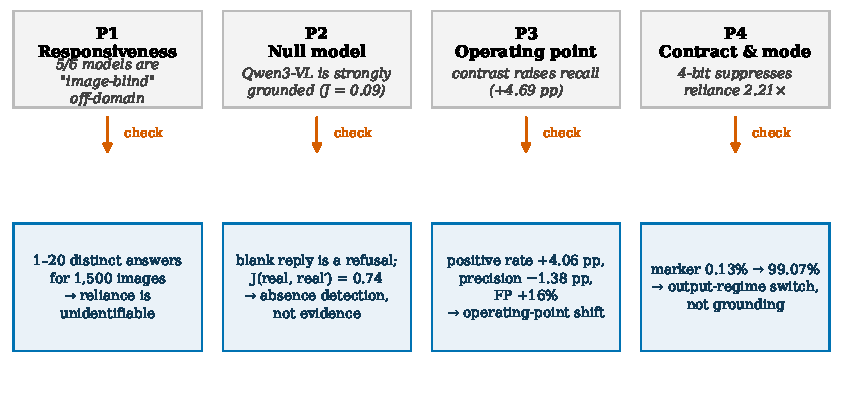
\includegraphics[width=\textwidth]{figures/fig01_four_reversals.pdf}
\caption{四个前提及其所防止的四次反转。上排是仅凭被报告统计量会得到的结论；下排是检查之后应得的结论。}
\label{fig:reversals}
\end{figure}

\section{相关工作}
\label{sec:related}

\textbf{反事实依赖。}\emph{To See or To Please}~\citep{anon2026see} 提出的 Visual Necessity Score 是最接近的先行工具：它在 full、blind、noise、conflict 四种条件下评测九个 VLM、9,000 个模型--样本对，并报告模型家族尺度规律与一种免训练的选择性预测增益。我们的依赖条件属于同一家族，但问题不同：不是``分数是多少''，而是``分数何时可识别''。该文的无图像对照没有报告真实图像间的零模型；我们表明这一省略可能反转排序（第~\ref{sec:results-null}~节）。\emph{Do VLMs See or Guess?}~\citep{anon2026guess} 固定图像、改变问题措辞，以隔离文本先验依赖。我们的结果与之互补：当图像被移除或退化时，坍缩或模板化的模型可以产生很大的表观对照，却没有证据提取，因此仅靠措辞控制不足以识别图像使用。

\textbf{退化鲁棒性。}医学 VLM 鲁棒性通常用干净误差与平均退化误差~\citep{anon2025corruption}，或用准确率与伪影检测率~\citep{cheng2025robustness} 来概括。这些指标在标签上聚合，因而看不到工作点移动：当真阳性与假阳性同时上升时，准确率可能不变甚至提高。我们对胸片 VLM 评测中的这一失效模式给出了明确的实证分析，表明退化可以\emph{提高}召回率，同时精确率与假阳性朝不利于鲁棒性的方向变化；要检测这一模式，两者都必须报告。压力测试套件报告了提示与工作流变化下的类似脆弱性~\citep{gu2025illusion}，接地研究则质疑医学 VLM 是否真正使用图像证据~\citep{felizzi2025grounded}。

\textbf{保守的默认正常行为。}\emph{Reliability Stress Tests}~\citep{anon2026stress} 表明，在提示与工作流变化下，精确匹配准确率会高估那些默认回答``正常''的保守模型，并以 CheXagent~\citep{chen2024chexagent} 与 MedGemma~\citep{sellergren2025medgemma} 为例。我们在更大规模上复现了这一现象，并加入契约轴：捷径的\emph{形式}（自信正常还是弃答）由回答模式决定，而不是由模型决定（第~\ref{sec:results-schema}~节）。我们的标签级分析还把``默认正常''与``输出坍缩''区分开来，而后者未被该框架区分。

\textbf{弃答与拒答。}\emph{Knowing When Not to Answer}~\citep{anon2026knowing} 评测不可回答的多模态输入上的弃答，并表明假设所有输入均可回答的基准会遗漏这一失效模式。我们的空白对照分析展示了一个互补的伪影：在散文契约下，对空白图像弃答很常见，除非检查空白模板，否则会产生虚假的``强依赖''读数（第~\ref{sec:results-null}~节）。

\textbf{推理长度与终止。}另一条工作线表明更长的推理并非单调更优：准确率随思维链长度呈倒 U 形~\citep{wu2026whenmore}，延长的思考可能放弃模型本来已经得到的答案~\citep{zhou2026overthinking}，而被截断的推理链可能比不推理更糟~\citep{su2026broken}。这些文献在固定预算下测量准确率。我们的第二模型结果是测量层面的后果：当推理检查点被要求输出结构化答案时，不终止会把该格子从分母中移除，因此覆盖率本身成为退化的函数（第~\ref{sec:results-second}~节）。

\textbf{校准与选择性预测。}校准通常用 ECE 度量、用温度缩放修正~\citep{guo2017calibration}，而它在分布偏移下的脆弱性已有充分记录~\citep{ovadia2019trust}。风险--覆盖率分析是医学机器学习的标准工具~\citep{geifman2017selective,oakdenrayner2021limits}。我们的贡献是具体而负面的：在预先声明的代价模型下，复合策略在图像级从不接受（接受率 0.000）；在发现级，它接受 17--41\% 的条目，但接受项误差率为 5.7--21.7\%，高于 5\% 预算。图像级 5\%/10\%/20\% 风险下的覆盖率均为 0.000；发现级覆盖率最多为 0.093。把 shift 或依赖信号加入置信度，最多使发现级 AUROC 变化 0.034，因此即便排序有所改善，也不能转化为可用的决策规则（第~\ref{sec:results-selective}~节）。

\textbf{报告生成与幻觉。}胸片报告生成除流畅度外，还以事实完整性与幻觉来评价~\citep{heiman2025factchexcker}。我们的 Open-i 层用一个刻意简单的标注器同时处理参考报告与生成报告；CheXbert 交叉核验表明漏报排序依赖标注器，而幻觉排序方向保持一致，因此我们只把后者作为稳定结果报告（第~\ref{sec:results-report}~节）。

\textbf{数据集与标签来源。}本文使用的公开胸片语料由弱监督与报告导出标签构建~\citep{wang2017chestxray8,bustos2020padchest,irvin2019chexpert,johnson2019mimic,chambon2024chexpertplus}。其标签噪声、站点构成与评测惯例限制了基准所能主张的范围~\citep{rafferty2026limitations}，而病理与站点之间的混杂可以在随机划分后继续存在~\citep{zech2018confounding}。监督胸片分类器（DenseNet、CheXNet）仍是判别力的参照~\citep{rajpurkar2017chexnet,huang2017densely}。为把模型弱点与任务固有难度分开，我们与 VLM 并行训练了一个患者不重叠的 DenseNet-121 基线（宏 AUROC 0.733；第~\ref{sec:results-baseline} 节）。因此我们把标签来源与病例构成当作测量声明，而不是事后补上的注意事项（表~\ref{tab:prevalence}）。

\textbf{医学基础模型与报告规范。}通用医学 AI 与医学 LLM 的动机是规模与广度~\citep{moor2023foundation,singhal2023medpalm,bommasani2021foundation}，但基准主张需要可追溯的数据与模型来源。数据表~\citep{gebru2021datasheets} 与模型卡~\citep{mitchell2019model} 是既有的记录工具；我们的四个前提是针对单个评测数字的、任务特定的同类契约。

\textbf{测量有效性与直接竞品。}若干 2026 年工作提出了相邻问题（表~\ref{tab:competitors}）。\emph{Answer, Clarify, or Abstain}~\citep{nguyen2026answer} 为医学 VLM 提出细粒度选择性预测；CALM-VLM~\citep{dhinagar2026calm} 把校准与选择性预测用于脑 MRI；两者都在输出层面行动，但没有审计测量前提。\emph{Beyond Accuracy}~\citep{zafar2026beyond} 评估多模态医学推理中的视觉 grounding；Buckley 等~\citep{buckley2026exploit} 表明多模态基础模型可能利用文本捷径做医学预测。Qu 等~\citep{qu2026accuracy} 在乳腺摄影中发现，回答准确率会高估证据接地与弃答可靠性；我们的胸片多标签协议加入响应性、真实图像间零模型、工作点与契约覆盖四项审计，并报告选择性可信的负结果。两项负结果也很接近：Fisher~\citep{fisher2025negative} 报告视觉语言基础模型可能无法迁移到 CXR 分类；AT-CXR~\citep{li2025atcxr} 提出不确定性感知的分诊。

\begin{table}[t]
\centering
\footnotesize
\setlength{\tabcolsep}{3pt}
\caption{与最接近的 2025--2026 工作的定位。``重叠''是该文已经建立的内容；``增量''是本文在其之外增加的内容。我们不主张任何单一组件为首创。}
\label{tab:competitors}
\begin{tabular}{@{}>{\raggedright\arraybackslash}p{0.19\textwidth}>{\raggedright\arraybackslash}p{0.22\textwidth}>{\raggedright\arraybackslash}p{0.25\textwidth}>{\raggedright\arraybackslash}p{0.24\textwidth}@{}}
\toprule
工作 & 主要问题 & 重叠 & 本文增量 \\
\midrule
\emph{To See or To Please}~\citep{anon2026see} & blind/noise/conflict 下的 VLM 依赖 & 依赖分数（VRS）、家族尺度 & 真实图像间零模型；响应性；工作点；契约覆盖 \\
\emph{Reliability Stress Tests}~\citep{anon2026stress} & 胸片 VLM 的提示/工作流压力测试 & 精确匹配高估默认正常 & 契约轴；三层；标签级与选择性指标 \\
\emph{Do VLMs See or Guess?}~\citep{anon2026guess} & 措辞控制的文本先验 & 无图像对照 & 坍缩/模板零模型；响应性审计 \\
\emph{Answer, Clarify, or Abstain}~\citep{nguyen2026answer} & 医学 VLM 的细粒度选择性策略 & 回答/澄清/弃答决策 & 负结果；策略可信前的四项前提 \\
\emph{Accuracy Overstates}~\citep{qu2026accuracy} & 乳腺摄影接地与弃答 & 准确率高估可靠性 & 胸片多标签；跨数据集层；工作点 \\
CALM-VLM~\citep{dhinagar2026calm} & 脑 MRI 校准 + 选择性预测 & 校准与选择性指标 & 胸片；契约覆盖；跨数据集坍缩 \\
AT-CXR~\citep{li2025atcxr} & 不确定性感知的胸片智能分诊 & 用于分诊的不确定性 & 审计测量，而非分诊策略 \\
VL FMs do not transfer~\citep{fisher2025negative} & 胸片分类的负迁移 & 迁移失败 & 机制：响应性与零模型；三层 \\
\bottomrule
\end{tabular}
\end{table}

我们的增量不是新分数或新策略，而是对响应性、零模型、工作点与契约覆盖的联合审计，以及发现级负结果：复合策略接受 17--41\% 的条目，但接受项误差率为 5.7--21.7\%，高于 5\% 预算。我们不主张任何单一组件的优先权。

\textbf{数据集与模型。}我们使用 NIH ChestX-ray14~\citep{wang2017chestxray8}、PadChest~\citep{bustos2020padchest} 与 Open-i~\citep{demnerfushman2016openi}，以及 Qwen2.5-VL~\citep{bai2025qwen25vl}、Qwen3-VL~\citep{qwen2025qwen3vl}、InternVL3.5~\citep{opengvlab2025internvl35}、MedGemma~\citep{sellergren2025medgemma} 与 CheXagent~\citep{chen2024chexagent}。LLaVA-Med~\citep{li2024llavamed} 单独运行，并因不遵守结构化契约而被排除在定量比较之外。

\section{协议}
\label{sec:protocol}

\subsection{模型与作为声明变量的精度}

我们评测来自四个家族的六个\emph{模式合规}模型，各按我们实际部署的精度运行：4-bit 为事后 NF4 量化，bf16/fp16 为发布精度；三个 4-bit 模型另做 bf16 对照（表~\ref{tab:models}）。模式合规与契约覆盖是两个概念：CheXagent 可以解析，但只覆盖 18.9\% 的标签槽位（第~\ref{sec:preconditions}~节）。LLaVA-Med-1.5-7B 单独运行：其散文输出不遵守 JSON 契约，\texttt{parse\_success=false} 是设计预期，其数字被排除在所有定量比较之外。

\begin{table}[t]
\centering
\small
\caption{模型与精度。``对照''是同一组四个依赖条件所使用的另一精度。}
\label{tab:models}
\begin{tabular}{llll}
\toprule
模型 & 家族 & 主精度 & 对照 \\
\midrule
MedGemma-4B-IT & MedGemma & 4-bit (NF4) & bf16 \\
MedGemma-1.5-4B-IT & MedGemma & 4-bit (NF4) & bf16 \\
Qwen2.5-VL-7B-Instruct & Qwen & 4-bit (NF4) & bf16 \\
Qwen3-VL-8B-Instruct & Qwen & bf16 & --- \\
InternVL3.5-8B & InternVL & bf16 & --- \\
CheXagent-8B & CheXagent & fp16 & --- \\
\bottomrule
\end{tabular}
\end{table}

\subsection{数据层}

\textbf{NIH（域内，结构化）。}1,506 例研究（\texttt{internal\_test} 1,054 + \texttt{source\_val} 452）。19 格网格：干净图像加六类退化（分辨率、噪声、模糊、JPEG、对比度、亮度），每类三个严重度，每个模型 28,614 个单元。真值来自 NIH 清单中的八标签多标签标注。

\textbf{病例构成。}NIH 评测集由分层采样器构建，刻意富集七个疾病标签，因此其阳性率高于 ChestX-ray14 的自然分布（肺不张 50.7\% 对 10.3\%；no-finding 8.0\% 对 53.8\%；附录~\ref{app:risk}，表~\ref{tab:prevalence}）。AUROC 在期望意义上不受患病率影响，但精确率与阳性预测率不是：这两者只在层内比较，绝不跨层比较。PadChest 保持其原生、稀疏得多的病例构成，因此跨数据集 $\Delta$AUROC 是在未匹配病例谱上得到的域统计量，需与第~\ref{sec:sensitivity}~节的共同标签分析一起解读。

\textbf{依赖条件。}四种条件——原图、空白（同尺寸均匀灰块）、强模糊、打乱图像——每个模型 6,024 个单元。空白是全篇使用的反事实。

\textbf{精度对照。}三个主实验为 4-bit 的模型在另一精度下重复同样四种依赖条件（每个 6,024 个单元）。

\textbf{模式消融。}五种回答模式 $\times$ \{原图, 空白\}，在 MedGemma-4B 上运行（15,060 个单元），仅改变所请求的输出契约。

\textbf{PadChest（跨医院，结构化）。}1,500 例研究，存储分辨率加空白对照（每个模型 3,000 个单元）。图像与标签均不重采样；PadChest 的 120 标签词表被映射到相同的八种发现，其中肺炎结构性缺失。固定处理器可能在模型内部降采样（表~\ref{tab:geometry}）。

\textbf{Open-i（报告生成，散文）。}947 例研究，原图与空白（每个模型 1,894 个单元）。参考报告由冻结的规则标注器打分（关键词加否定窗口），并在每条输出中记为 \texttt{evidence\_method}。

表~\ref{tab:calls} 汇总调用预算：六模型矩阵共 \textbf{270,324 次模型调用}，加上 LLaVA-Med 实验的 5,294 次，共 275,618 次。

\begin{table}[t]
\centering
\small
\caption{数据层、每模型单元数与总调用量。}
\label{tab:calls}
\begin{tabular}{llrr}
\toprule
数据层 & 阶段 & 每模型单元数 & 模型数 \\
\midrule
NIH & shift（19 格网格） & 28,614 & 6 \\
NIH & 依赖（4 条件） & 6,024 & 6 \\
NIH & 精度对照 & 6,024 & 3 \\
NIH & 模式消融 & 15,060 & 1 \\
PadChest & 原生 + 空白 & 3,000 & 6 \\
Open-i & 报告 + 空白 & 1,894 & 6 \\
NIH & LLaVA-Med 子集 & 400 & 1 \\
\midrule
\multicolumn{2}{l}{合计（含 LLaVA-Med 5,294）} & \multicolumn{2}{r}{275,618 次调用} \\
\bottomrule
\end{tabular}
\end{table}

\subsection{冻结的测量选择}

所有模型使用贪婪解码（\texttt{do\_sample=False}，单束）、每层单一提示模板与同一解析器。每张图像按存储分辨率送入，直至各模型声明的上限；固定处理器可能在模型内部降采样（表~\ref{tab:geometry}），因此``全分辨率''是模型相关的，而不是共享设置。各模型的有效输入几何因架构而异，作为测量的一部分记录，而不是当作中性设置。在最大的 PadChest 图像（15.37\,MP）上，Qwen3-VL 接收 15.24\,MP，Qwen2.5-VL 接收 12.85\,MP（其检查点上限），MedGemma 接收 0.80\,MP，InternVL/CheXagent 接收 0.20\,MP。因此，跨家族比较的是``同一张图像经过六条不同输入路径''；我们明确报告这一点，而不是把它当作可忽略的干扰。

\subsection{评估口径}

两个层级严格分开。\emph{描述性输出分析}——响应性、干净与退化准确率、工作点变化、契约与报告指标——使用全部 1,506 例 NIH 研究，因为它们不拟合任何参数：每个数字都是冻结输出与标签的函数。\emph{拟合策略分析}——校准温度、风险阈值与三动作策略——所有参数都在 \texttt{source\_val}（452 例）上拟合，只在 \texttt{internal\_test}（1,054 例研究、8,432 个发现项、427 个患者簇）上报告。表~\ref{tab:clean} 与表~\ref{tab:op} 属于第一层；表~\ref{tab:selective} 与图~\ref{fig:selective}--\ref{fig:risk} 属于第二层。第二层中没有任何数字包含用于拟合其阈值的研究。

\subsection{统计}

比例使用 Wilson 95\% 区间。AUROC 与风险--覆盖率区间使用患者聚类自助法（1,000 次重采样）。单位是研究（一张图像）：每例研究带有源元数据中的患者标识，重采样抽取患者，因此同一患者的所有图像一起移动。干净与退化行按研究标识连接，使每例研究同时进入两种条件。工作点指标由模型实际输出的状态计算，而不是来自拟合切点：``positive'' 即模型自己的决策。0.5 概率切点只用于没有显式状态的槽位，校准概率只用于上一节所述的拟合层。校准与决策阈值只在 \texttt{source\_val} 上拟合、在 \texttt{internal\_test} 上评估。我们不对 $n=5$ 或 $n=6$ 拟合模型级回归；跨模型一致性以两两秩相关报告；任何用于\emph{描述性}划分的阈值都标注为``描述性，非拟合''。

\section{四个前提}
\label{sec:preconditions}

把每个被报告的量写成 $M=f(\text{模型},\text{数据},\text{干预},\text{契约},\text{决策规则})$。只有当设计钉住了目标量所依赖的每一个自变量，该指标才是\emph{可识别}的。表~\ref{tab:framework} 对每个前提给出目标量、识别条件、违反时的失效模式、审计统计量，以及审计通过后仍被允许的最强主张。下面的小节定义这些统计量；该表是可复用的对象。

我们是在弱的、审计意义上使用``识别''一词：若在固定模型的前提下改变测量设计不会系统性地改变该统计量的符号、分母或解释，则该统计量对其目标量是已识别的。这不是充要刻画。阈值（众数占比 0.50、唯一回答 5）是可操作的启发式，而不是证明；第~\ref{sec:sensitivity}~节对其做扫描，并且正文写明审计失败时仍被允许的主张是什么。四个条件是有序的，而不是并列的：P4 固定输出空间及其分母，P1 确认真实图像上的输出支撑集非退化，P2 在该空间中检验分离度，P3 只在已声明或固定的决策规则下才允许鲁棒性主张。

\begin{table}[H]
\centering
\footnotesize
\setlength{\tabcolsep}{3pt}
\begingroup\hyphenpenalty=10000
\caption{四个前提作为识别条件。每行说明：要估计什么；被报告的数字要识别它必须满足什么；条件失败时数字会被怎样误读；用什么统计量审计；以及仍被允许的主张。}
\label{tab:framework}
\begin{tabular}{@{}>{\raggedright\arraybackslash}p{0.135\textwidth}>{\raggedright\arraybackslash}p{0.13\textwidth}>{\raggedright\arraybackslash}p{0.18\textwidth}>{\raggedright\arraybackslash}p{0.17\textwidth}>{\raggedright\arraybackslash}p{0.15\textwidth}>{\raggedright\arraybackslash}p{0.16\textwidth}@{}}
\toprule
前提 & 目标量 & 识别条件 & 违反时的失效模式 & 审计统计量 & 允许的主张 \\
\midrule
P1 响应性 & 可归因于图像变化的输出变异 & 真实输入上的输出支撑非退化 & 常数或模板输出使一切对照不可识别 & 唯一回答数；众数占比及 Wilson 区间；空白模板占比 & ``无可测响应''，而非``零依赖'' \\
P2 零模型 & 干预下的证据特异性偏离 & 同空间分离 $\Delta_{\text{null}}$ 超过零 & 拒答或样板文本伪装成很大的对照 & $D(\text{真实},\text{空白}) - D(\text{真实},\text{真实}')$\newline 其中 $D_{\text{text}}=1-J$，$D_{\text{prob}}=\text{mean}\,|\Delta P|$ & ``对照超过自然变异''，而非``提取了证据'' \\
P3 工作点 & 被恢复证据的变化 & 在已声明的决策规则下，召回率与阳性预测率、精确率并读 & 移动的工作点被读作鲁棒性提升 & $\Delta$召回率、$\Delta$阳性预测率、$\Delta$精确率、病例级转移 & ``工作点移动''；只有规则固定时才可谈鲁棒性 \\
P4 契约覆盖 & 已覆盖槽位上的临床正确性 & 契约覆盖与输出模式已声明且可比 & 分母或输出体制在单元间改变 & 确定状态槽位占比；状态分布；标记与概率完整度 & 只在同一契约与输出体制内可比 \\
\bottomrule
\end{tabular}
\endgroup
\end{table}

\subsection{P1——响应性：模型在真实图像上是否有变化？}

把一个模型在某个数据层上的\textbf{输出支撑大小}定义为 $N$ 张真实图像上不同归一化回答的数量，把\textbf{众数占比}定义为众数回答的频率，并给出 Wilson 区间。只有当模型不是常数函数时，依赖对照才可解释。我们以描述性方式操作化该检查：$\text{众数占比} \ge 0.50$ 或 $\text{唯一回答数} \le 5$ 标记输出坍缩。规则在分析前声明，且从不过滤数据。

\subsection{P2——零模型：没有干预时对照会是多少？}

对每一个真实图像与干预图像的对照，在同一度量空间中报告两张\emph{不同真实}图像之间的同一统计量——真实图像间零模型。文本用 $D_{\text{text}} = 1-J$；结构化输出用八个标签上的 $D_{\text{prob}} = \text{mean}\,|\Delta P|$。两者都是距离，因此可解释的量是二者之差，即\textbf{分离}
\[
\Delta_{\text{null}} = D(\text{真实},\text{空白}) - D(\text{真实},\text{另一真实}).
\]
\begin{itemize}[leftmargin=1.2em,itemsep=1pt,topsep=2pt]
\item $\Delta_{\text{null}} > 0$：干预比一张随机真实图像\emph{更远}（存在一定分离）；
\item $\Delta_{\text{null}} \approx 0$：干预与随机真实图像不可区分（没有证据）；
\item $\Delta_{\text{null}} < 0$：干预比随机真实图像\emph{更近}（模型用先验作答）。
\end{itemize}
两个空间共用同一符号约定很重要：Jaccard 是相似度，而 $|\Delta P|$ 是距离，若比较两个空间的原始``差距''，正值含义会被翻转。

\subsection{P3——工作点：决策阈值发生了什么？}

同时报告阳性召回率、阳性预测率与精确率。没有阳性预测率的召回变化，无法区分``恢复了更多证据''与``阈值移动了''。

\subsection{P4——契约覆盖与输出模式}

报告 (a) 具有确定状态（阳性或阴性）的标签槽位比例，并与 uncertain 与未提及状态分开；以及 (b) 当两次运行跨精度或跨提示比较时，报告输出模式指示量——推理通道触发率、概率完整度。在 19\% 槽位上计算的指标，与在 99\% 槽位上计算的指标不可比。

\subsection{契约术语}

四个量在全文中严格区分。\textbf{模式合规}问回答能否解析为所请求的格式。\textbf{契约覆盖}问有多大比例的标签槽位带有确定状态（阳性或阴性），而非 \texttt{uncertain} 或 \texttt{not\_mentioned}。\textbf{临床正确性}问这些确定状态是否与参考标签一致。\textbf{弃答}问模型是否明确拒绝（\texttt{uncertain} 状态或拒答句）。一个模型可以完全模式合规却只覆盖 19\% 的槽位；可以弃答而不违反任何模式；散文模型则可以既不合规也不被覆盖。混淆这四者是不可比数字最常见的来源，因此下文每个指标都写明其分母。

\subsection{审计}

表~\ref{tab:audit} 把 P1--P2 应用于三个数据层。实现为 \url{scripts/78_responsiveness_audit.py}（仅 CPU）与 \url{scripts/79_export_selective_inputs.py}。坍缩规则是描述性的，从不过滤；第~\ref{sec:sensitivity}~节对其做扫描，表明核心跨数据集结论在众数占比阈值直至 0.80 时仍成立。

\begin{table}[t]
\centering
\footnotesize
\caption{响应性审计（全量数据）。六个模式合规模型覆盖三个数据层，另加 LLaVA-Med 在 PadChest、Open-i 与一个 200 例 NIH 子集上的运行。唯一回答数 = $N$ 张真实图像上不同归一化回答的数量。零模型统计量为\emph{分离} $\Delta_{\text{null}} = D(\text{真实},\text{空白}) - D(\text{真实},\text{另一真实})$，其中 $D_{\text{text}} = 1-J$、$D_{\text{prob}} = \text{mean}\,|\Delta P|$；正值表示干预比随机真实图像离真实图像更远（存在分离），负值表示更近（先验或样板）。众数占比的 Wilson 区间为 $\pm\le 0.02$，为节省篇幅省略。$\dagger$ LLaVA-Med 的空白回答为空，真实-空白 Jaccard 无定义；该统计量记为 n/a，而不是作为对照解释。}
\label{tab:audit}
\begin{tabular}{llrrrrcrr}
\toprule
数据层 & 模型 & $N$ & 唯一回答 & 众数占比 & 坍缩 & $\Delta_{\text{null}}$（文本） & $\Delta_{\text{null}}$（概率） \\
\midrule
NIH & MedGemma-4B & 1,506 & 336 & 0.052 & 否 & $+0.006$ & $+0.131$ \\
NIH & MedGemma-1.5 & 1,506 & 250 & 0.099 & 否 & $+0.867$ & $+0.007$ \\
NIH & InternVL3.5 & 1,506 & 313 & 0.161 & 否 & $+0.025$ & $+0.041$ \\
NIH & Qwen3-VL & 1,506 & 125 & 0.547 & \textbf{是} & $-0.009$ & $-0.066$ \\
NIH & CheXagent & 1,506 & 10 & 0.687 & \textbf{是} & $-0.070$ & n/a \\
NIH & Qwen2.5-VL & 1,506 & 6 & 0.986 & \textbf{是} & $0.000$ & $-0.001$ \\
NIH & LLaVA-Med（子集） & 200 & \textbf{2} & 0.987 & \textbf{是} & n/a$^{\dagger}$ & n/a \\
\midrule
PadChest & MedGemma-4B & 1,500 & \textbf{20} & 0.903 & \textbf{是} & $-0.002$ & $-0.009$ \\
PadChest & MedGemma-1.5 & 1,500 & 329 & 0.373 & 否 & $+0.206$ & $+0.134$ \\
PadChest & InternVL3.5 & 1,500 & \textbf{2} & 0.892 & \textbf{是} & $-0.006$ & $0.000$ \\
PadChest & Qwen3-VL & 1,500 & \textbf{3} & 0.998 & \textbf{是} & $0.000$ & $-0.000$ \\
PadChest & CheXagent & 1,500 & 3 & 0.983 & \textbf{是} & $-0.002$ & n/a \\
PadChest & Qwen2.5-VL & 1,500 & \textbf{1} & 1.000 & \textbf{是} & $0.000$ & $0.000$ \\
\midrule
Open-i & MedGemma-4B & 947 & 78 & 0.604 & \textbf{是} & $-0.070$ & n/a \\
Open-i & MedGemma-1.5 & 947 & 275 & 0.300 & 否 & $-0.087$ & n/a \\
Open-i & InternVL3.5 & 947 & 222 & 0.243 & 否 & $+0.112$ & n/a \\
Open-i & Qwen3-VL & 947 & 109 & 0.326 & 否 & $+0.648$ & n/a \\
Open-i & CheXagent & 947 & 85 & 0.265 & 否 & $-0.030$ & n/a \\
Open-i & Qwen2.5-VL & 947 & 218 & 0.226 & 否 & $+0.193$ & n/a \\
\midrule
PadChest & LLaVA-Med & 1,500 & 19 & 0.591 & \textbf{是} & n/a$^{\dagger}$ & n/a \\
Open-i & LLaVA-Med & 947 & \textbf{2} & 0.671 & \textbf{是} & $-0.059$ & n/a \\
\bottomrule
\end{tabular}
\end{table}

由此可得到三个事实。(i) 坍缩并不局限于域外数据层：Qwen2.5-VL 与 CheXagent 在域内也是常数机器。(ii) 在域内具有响应性的模型可以在域外坍缩：MedGemma-4B 336$\rightarrow$20、InternVL3.5 313$\rightarrow$2、Qwen3-VL 125$\rightarrow$3；只有 MedGemma-1.5 保持（250$\rightarrow$329）。(iii) 正的文本分离不是 grounding 的证据：Qwen3-VL 的 $+0.648$ 来自拒答模板，Qwen2.5-VL 的 $+0.193$ 来自第二条样板文本。图~\ref{fig:resp} 展示了该审计。

\section{结果}
\label{sec:results}

\subsection{准确率低于平凡上限，判别力处于随机水平}
\label{sec:results-accuracy}

在 NIH 干净单元上，七个病理标签（七个全阴；排除 \texttt{no\_finding}）的多数类上限为标签槽位的 \textbf{0.6579}。没有模型超过该上限 1.0\,\pp{} 以上；最好的 InternVL3.5（0.6674）为 +0.95\,\pp{}，Qwen2.5-VL（0.6578）甚至\emph{低于}上限。所有模型的干净 AUROC 为 0.50--0.63（表~\ref{tab:clean}）。以准确率优先的报告会把这张表描述为``0.54--0.67 的准确率''；加入上限后，同一张表说明的是``任何地方都没有可用的判别力''。该主张的监督复现在第~\ref{sec:results-baseline} 节。

\begin{table}[t]
\centering
\small
\caption{NIH 干净性能与七病理标签上的全阴上限（排除 \texttt{no\_finding}；$n=1{,}506$ 例研究，10,542 个病理槽位）。上限在每个模型的确定槽位上计算：0.6579；CheXagent 为 0.6570，因为它只有 18.9\% 的槽位具有确定状态。宏 AUROC 为七个病理标签上的患者聚类自助法 95\% 区间（1,000 次重采样；缺失概率按 0.0 计，与脚本 75 一致）。}
\label{tab:clean}
\begin{tabular}{lrrrrr}
\toprule
模型 & 合并准确率 & 相对上限 & 宏平均 AUROC [95\% CI] & 宏平均 ECE & 阳性召回率 \\
\midrule
InternVL3.5 & 0.6674 & $+1.0$\,\pp{} & 0.6066 [0.5949, 0.6191] & 0.247 & 0.4928 \\
MedGemma-1.5 & 0.6106 & $-4.7$\,\pp{} & 0.5852 [0.5748, 0.5952] & 0.234 & \textbf{0.6392} \\
MedGemma-4B & 0.5398 & $-11.8$\,\pp{} & 0.6270 [0.6138, 0.6394] & 0.207 & 0.5519 \\
Qwen3-VL & 0.5926 & $-6.5$\,\pp{} & 0.5455 [0.5350, 0.5568] & 0.348 & 0.1625 \\
Qwen2.5-VL & 0.6578 & $\mathbf{-0.01}$\,\pp{} & 0.5013 [0.5003, 0.5027] & 0.412 & 0.0039 \\
CheXagent & 0.0589 & $-59.8$\,\pp{} & 0.5001 [0.5000, 0.5002] & 0.310 & 0.0003 \\
\bottomrule
\end{tabular}
\end{table}

宏 ECE 作为描述性的可靠性摘要报告，而不是校准主张：概率以文字形式写在回答里，只对确定槽位存在，CheXagent 根本没有概率通道，也未做任何事后校准。因此本表中只有 AUROC 一列是六个模型间可比的判别量。

\subsection{退化可以通过移动工作点提高召回率}
\label{sec:results-op}

表~\ref{tab:op} 报告合并层面的重度对干净变化。工作点案例是那些干净阳性预测率较高的模型；基线很低的模型没有向上移动的空间。这是\emph{测量体制}的性质，而不是``退化无害''的主张：两个 InternVL3.5 行的精确率下降（$-1.38$ 与 $-0.64$\,\pp{}），Qwen3-VL 的精确率略升（$+0.19$\,\pp{}），而三个单元的阳性预测率都上升，假阳性分别增加 16\%、8\% 与 20\%。InternVL3.5 对比度单元的增加集中在肺炎（$+98$）与实变（$+69$），占 259 例新增假阳性的 64.5\%，气胸为 0（表~\ref{tab:flip}）。患者聚类自助法（1,000 次重采样；\url{scripts/85_operating_point_ci.py}）给出三个单元的 $\Delta$召回率：$+4.69$ $[3.75,5.56]$、$+2.52$ $[1.46,3.63]$、$+3.44$ $[2.37,4.69]$\,\pp{}；$\Delta$阳性预测率：$+4.06$ $[3.44,4.64]$、$+2.09$ $[1.36,2.85]$、$+2.51$ $[1.75,3.26]$；所有区间都排除零。精确率变化只有 InternVL3.5 对比度单元排除零（$-1.38$ $[-2.16,-0.63]$\,\pp{}）；另外两个区间包含零。对 InternVL3.5 对比度单元，病例级转移（附录~\ref{app:risk}，表~\ref{tab:flip}）显示的是广泛重分类，而不是有针对性地找回丢失发现；下文的固定规则重跑表明分数分布本身在移动，因此我们把该模式标记为\emph{工作点移动}，而不是已被证明的阈值变化。对输出的概率做事后固定 $0.5$ 切点，可复现同样的变化（对比度 $+4.80$ 对 $+4.69$\,\pp{}，亮度 $+2.47$ 对 $+2.52$\,\pp{}，Qwen3-VL $+3.36$ 对 $+3.44$\,\pp{}；附录~\ref{app:risk}，表~\ref{tab:fixedthr}），因此该移动不是离散状态规则改变造成的伪影。它仍是工作点移动，因为概率尺度本身发生了移动。真正的固定规则重跑确认了这一点：只要求模型输出概率、由我们在 0.5 处赋状态，对比度 severe 使召回由 0.510 升至 0.575、阳性率由 0.404 升至 0.449，亮度 severe 使召回升至 0.584、阳性率升至 0.457（200 例配对研究；附录~\ref{app:risk} 表~\ref{tab:fixedrerun}）。由于该运行的决策规则不可能移动，增益来自分数分布移动，而不是离散状态规则改变。第二个推理模型以相反方向复现了该工作点机制（第~\ref{sec:results-second} 节）。反转 3 也不需要语言模型：同一个 DenseNet-121 检查点在 19 格网格上以固定 0.5 规则运行，对比度 severe 下合并召回由 0.567 升至 0.588、阳性率由 0.360 升至 0.378，而宏 AUROC 保持 0.733 $\rightarrow$ 0.729；噪声 severe 使召回降至 0.477、阳性率降至 0.321，分辨率 severe 降至 0.523 与 0.355（附录~\ref{app:risk} 表~\ref{tab:densenetgrid}）。因此机制是分数分布在移动，而不是文字状态在移动；模型间不同的是移动幅度（InternVL3.5 为 +4.7\,\pp{}，DenseNet 为 +2.1\,\pp{}）。

\begin{table}[t]
\centering
\small
\caption{重度对干净，七个病理标签合并（$n=1{,}506$；10,542 个病理槽位）。}
\label{tab:op}
\begin{tabular}{llrrrrl}
\toprule
模型 & 退化 & $\Delta$ 召回 & $\Delta$ 精确率 & $\Delta$ 阳性率 & 假阳性 & 判定 \\
\midrule
InternVL3.5 & 对比度 & $\mathbf{+4.69}$\,\pp{} & $-1.38$\,\pp{} & $\mathbf{+4.06}$\,\pp{} & 1,646 $\rightarrow$ 1,905 & 工作点移动 \\
InternVL3.5 & 亮度 & $+2.52$\,\pp{} & $-0.64$\,\pp{} & $+2.09$\,\pp{} & 1,646 $\rightarrow$ 1,775 & 工作点移动 \\
Qwen3-VL & 对比度 & $+3.44$\,\pp{} & $+0.19$\,\pp{} & $+2.51$\,\pp{} & 696 $\rightarrow$ 837 & 工作点移动 \\
MedGemma-1.5 & 对比度 & $+0.78$\,\pp{} & $+0.20$\,\pp{} & $+0.36$\,\pp{} & 2,425 & 稳定 \\
MedGemma-4B & 对比度 & $-1.66$\,\pp{} & $-0.40$\,\pp{} & $-0.87$\,\pp{} & 2,168 & 稳定 \\
MedGemma-1.5 & 分辨率 & $\mathbf{-18.77}$\,\pp{} & $-1.43$\,\pp{} & $-12.21$\,\pp{} & 1,786 & 召回损失 \\
MedGemma-4B & 噪声 & $\mathbf{-22.99}$\,\pp{} & $-0.09$\,\pp{} & $-16.51$\,\pp{} & 1,288 & 召回损失 \\
\bottomrule
\end{tabular}
\end{table}

\subsection{两个可分离的轴：可察觉性与损伤}
\label{sec:results-twoaxis}

对 MedGemma-1.5，推理通道触发率（以 \texttt{<unused94>thought} 开头的回答）是我们的操作化、\emph{基于标记}的读数：它记录模型是否进入与``注意到退化图像''相关的推理模式，而不表示模型是否具有该退化的内部表征。在 19 格网格上，基于标记的可察觉性按退化类别分离，而损伤并不跟随它（表~\ref{tab:twoaxis}）。

\begin{table}[t]
\centering
\small
\caption{基于标记的可察觉性与损伤（MedGemma-1.5，重度）。损伤排名把干净单元记为第 1 名，再按带符号的召回变化排列六个重度退化（最有害者在前）；可察觉性排名按标记率排列六个重度退化（最高者在前）。该标记是模型侧信号，不是图像侧可见性的度量。}
\label{tab:twoaxis}
\begin{tabular}{lrrrr}
\toprule
退化 & 标记率（重度） & 重度 $\Delta$ 召回 & 损伤排名 & 可察觉性排名 \\
\midrule
分辨率 & \textbf{71.98\%} & $-18.77$\,\pp{} & 2 & 1 \\
噪声 & \textbf{0.46\%} & $-17.22$\,\pp{} & 3 & 5 \\
模糊 & 29.35\% & $-5.10$\,\pp{} & 5 & 2 \\
JPEG & 27.42\% & $-9.03$\,\pp{} & 4 & 3 \\
对比度 & 0.60\% & $+0.78$\,\pp{} & 7 & 4 \\
亮度 & 0.20\% & $-1.19$\,\pp{} & 6 & 6 \\
\bottomrule
\end{tabular}
\end{table}

可察觉性与损伤之间的秩相关不是重点；重点是\emph{非对角线}。对 MedGemma-1.5——矩阵中唯一具有可读推理通道的模型——噪声造成的损伤与分辨率损失相当（$-17.2$ 对 $-18.8$\,\pp{}），而标记触发率低 \textbf{156 倍}（0.46\% 对 71.98\%）。其余五个模型不暴露该通道，其标记率结构性为 0，因此我们不做跨模型标记平均，也不把双轴结果解释为跨模型证据。在这一单模型范围内，结果是\textbf{静默失效象限}（图~\ref{fig:silent}）：一种破坏证据却不触发模型自监控信号的退化。对于监视推理通道激活或 token 级犹豫的部署监控器，噪声是看不见的。

两个控制排除了伪影。第一，\texttt{marker\_unparsed}（模型打开了通道却未能闭合 JSON）在整个网格上 $\le 1.20\%$，因此标记不是截断的代理。第二，干净单元只有 0.13\% 的回答打开通道，因此标记并非无条件出现。

第三个控制把失效定位在模型侧而非图像侧。在 1,506 张域内评估图像上，单一无参考统计量（Laplacian 方差）把干净图像与重度噪声图像分开的 AUC 为 $1.000$；高频能量的中位数从 $0.0011$ 升至 $0.0844$（附录~\ref{app:risk}，表~\ref{tab:imageside}）。同一统计量以相反方向把干净图像与重度模糊图像分开，AUC 同样为 $1.000$。因此，退化对通用图像质量监控器而言一目了然；失效的是模型自身的自监控通道。这把主张收窄到我们真正辩护的那一条：模型的监控信号没有登记一种会损害其答案的退化。该轴对的跨模型检验见第~\ref{sec:results-second} 节。

第四个基于规则的检查问：模型是否会\emph{用文字}说出来，而不是通过标记。在原始回答中搜索显式质量词（noise、degraded、quality、artifact、blur），六个模型在重度噪声下均为 \textbf{0.00\%}；MedGemma-1.5 在重度分辨率下为 3.85\%（58/1,506）；其他模型在该单元均不超过 0.00\%（\url{scripts/83_quality_language_audit.py}）。低标记率并没有被显式语言补偿。

\begin{figure}[t]
\centering
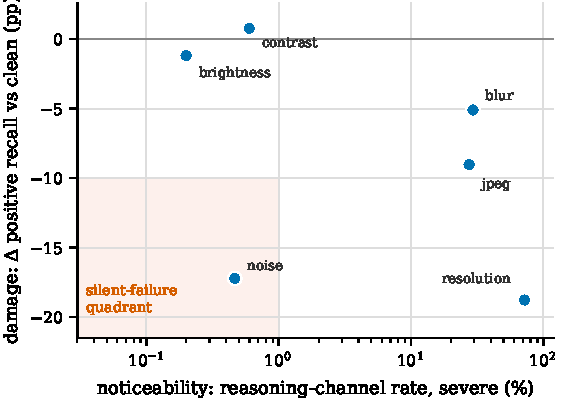
\includegraphics[width=0.62\textwidth]{figures/fig03_silent_failure.pdf}
\caption{静默失效象限（MedGemma-1.5，矩阵中唯一具有可读推理通道的模型）。基于标记的可察觉性是重度退化下的推理通道触发率；损伤是合并阳性召回的变化。阴影区域为低可察觉性且损伤显著；噪声落在其中。}
\label{fig:silent}
\end{figure}

\subsection{契约决定捷径的形式}
\label{sec:results-schema}

在模型、提示内容与空白图像固定的条件下，五种模式产生两种互不相交的失效形式（表~\ref{tab:schema}）。四种模式产生 \textbf{0/1,506} 条模式合规的空白回答，且都把 \texttt{no\_finding} 以概率 1.0 判为阳性。带 \texttt{uncertain} 状态的逐标签模式产生 \textbf{1,506/1,506} 条合规回答，75\% 的槽位弃答，\texttt{no\_finding} 阳性率为 0\%。两者的 Wilson 区间不重叠。

\begin{table}[t]
\centering
\small
\caption{模式消融，MedGemma-4B（每单元 $n=1{,}506$）。}
\label{tab:schema}
\begin{tabular}{lrrrr}
\toprule
模式 & 空白合规数 & 空白 \texttt{no\_finding} 阳性 & 真实召回 & 空白弃答率 \\
\midrule
v0 简单 & 0/1,506 & 1.000 & \textbf{0.499} & 0\% \\
v1 逐标签二分类 & \textbf{1,506/1,506} & 0.000 & 0.442 & \textbf{75\%} \\
v2 few-shot & 0/1,506 & 1.000 & 0.269 & 0\% \\
v3 报告优先 & 0/1,506 & 1.000 & 0.315（22.3\% 不可解析） & 0\% \\
v4 正常性压力 & 0/1,506 & 1.000 & \textbf{0.166} & 0\% \\
\bottomrule
\end{tabular}
\end{table}

同一实验反转了对提示敏感性的通常解读：产生最佳\emph{真实图像}召回的模式（v0），正是产生最自信\emph{空白图像}断言的那个模式。因此，``提示调优''与``grounding 诊断''不能互相替代。第二个医学模型上的复现与措辞对照见第~\ref{sec:results-schema2}~与~\ref{sec:results-paraphrase} 节。

\subsection{响应性在域外坍缩}
\label{sec:results-collapse}

表~\ref{tab:audit} 展示了坍缩；这里我们检验最明显的混杂。PadChest 的疾病阳性率低于 NIH（17.7\% 的研究至少含一个疾病标签，NIH 为 92.0\%；其余 NIH 研究仅含 no-finding），因此``永远回答正常''在 PadChest 上是更好的先验。限制到 \textbf{265 例疾病阳性研究}，六个模型中仍有五个坍缩：MedGemma-4B 8 种（众数 90.6\%）、InternVL3.5 2 种（89.4\%）、Qwen3-VL 2 种（99.6\%）、CheXagent 2 种（95.5\%）、Qwen2.5-VL 1 种（100\%）；只有 MedGemma-1.5 保持 91 种（34.7\%）。一个对其疾病阳性研究只给出一种回答的模型不是``保守''，而是没有响应性，其空白对照不可识别（图~\ref{fig:resp}）。这也解释了跨数据集迁移结果：常数函数按构造 AUROC 为 0.5。两个观察是同一事实的两次呈现。

\textbf{第七个模型：只在散文层运行。}LLaVA-Med 在 PadChest、Open-i 与一个 200 例 NIH 子集上运行，未跑完整的 28,614 单元网格，因为该子集已经显示同样的常数模板。它是一个\emph{双模板}模型：在 1,500 例 PadChest 研究上给出 19 种不同回答，其中 59.1\% 为同一模板、23.3\% 为空字符串、2.1\% 为安全免责声明；其 PadChest 空白回答 100\% 为空。在 Open-i 上它只给出两种回答：67.05\% 为``该胸片似乎无法判读''，32.95\% 为一句固定正常描述，任何研究都没有发现级内容。在 NIH 子集上它同样只给出两种回答，其中一种占 98.7\%，结构化解析率为 0\%，空白回答为空。因此，我们把它报告为\emph{实测}排除，而不是设计排除，并且不在发现层面给它打分（表~\ref{tab:audit}）。

\begin{figure}[t]
\centering
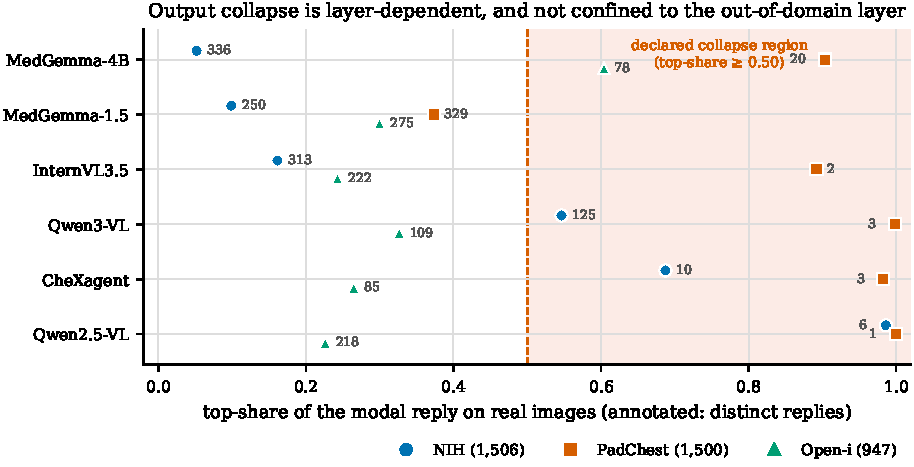
\includegraphics[width=\textwidth]{figures/fig02_responsiveness.pdf}
\caption{三个数据层上的响应性。每个标记是真实图像上众数回答的占比；旁边的数字是不同回答的数量。阴影区域是预先声明的坍缩规则。}
\label{fig:resp}
\end{figure}

\subsection{没有零模型的空白对照不是依赖度量}
\label{sec:results-null}

每个模型的空白回答都坍缩到极小的模板集合——五个模型为 1--2 种，Qwen2.5-VL 为 11 种样板变体，其中众数变体占 39.7\%。对 Qwen3-VL 与 CheXagent，该模板是\textbf{拒答}（``该研究无法判读……''，分别占空白回答的 96.3\% 与 100\%）；对其他四个模型，它是\textbf{通用正常报告}。在每种情况下，正确的零点是真实图像间相似度，而不是零相似度（表~\ref{tab:blanknull}，图~\ref{fig:null}）。

\begin{table}[t]
\centering
\small
\caption{Open-i 空白对照及其真实图像间零模型（$n=947$）。$\Delta_{\text{null}} = J(\text{真实},\text{另一真实}) - J(\text{真实},\text{空白})$ 即第~\ref{sec:preconditions}~节的距离型分离：正值表示空白回答比随机真实回答离真实回答更远。}
\label{tab:blanknull}
\begin{tabular}{lrrrl}
\toprule
模型 & $J(\text{真实},\text{空白})$ & $J(\text{真实},\text{另一真实})$ & $\Delta_{\text{null}}$ & 空白模板 \\
\midrule
CheXagent & 0.277 & 0.247 & $-0.030$ & 拒答 \\
Qwen3-VL & 0.091 & 0.740 & $+0.648$ & 拒答 \\
Qwen2.5-VL & 0.576 & 0.770 & $+0.193$ & 第二样板 \\
InternVL3.5 & 0.562 & 0.673 & $+0.112$ & 通用正常 \\
MedGemma-1.5 & 0.736 & 0.648 & $-0.087$ & 通用正常 \\
MedGemma-4B & 0.894 & 0.824 & $-0.070$ & 通用正常 \\
\bottomrule
\end{tabular}
\end{table}

原始 Jaccard 所暗示的排序（Qwen3-VL 最 grounded，MedGemma-4B 最差）在检查模板后不成立。最纯粹的案例是 LLaVA-Med：其 67.05\% 的真实 Open-i 回答与空白拒答逐字节相同，其余 32.95\% 是一句正常描述——两个模板，没有发现。PadChest 上的坍缩不是空字符串造成的伪影：只看 1,150 条非空回答，仍有 18 种不同字符串，众数占 77.0\%。结构化层同样如此：六个模型的空白回答都坍缩为一个 JSON 模板。概率空间分离是唯一能区分结构化模型的统计量，而且只区分三个：MedGemma-4B（NIH $+0.131$）、InternVL3.5（NIH $+0.041$）、MedGemma-1.5（PadChest $+0.134$）。对其他每个模型--数据层单元，正确的报告是``无可测效应''，而不是``零依赖''。

\begin{figure}[t]
\centering
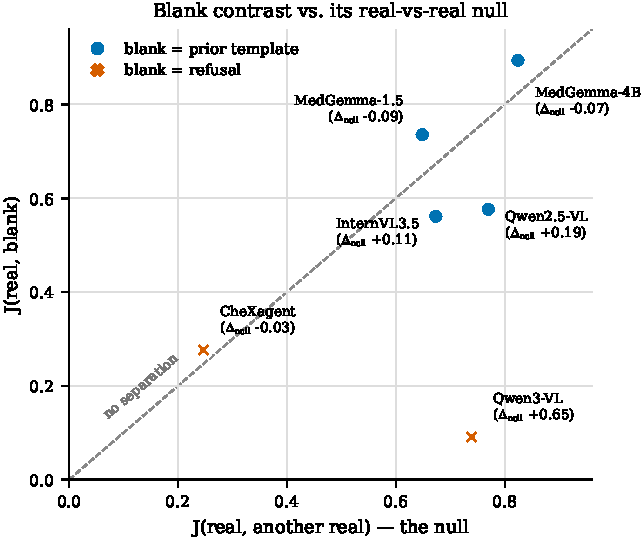
\includegraphics[width=0.62\textwidth]{figures/fig05_blank_null.pdf}
\caption{空白对照与其自身零模型。对角线上的点没有分离；对角线以下的点比随机真实报告更不同。拒答（叉号）远在对角线下方，但它测量的是缺失检测，不是证据提取。}
\label{fig:null}
\end{figure}

\subsection{精度改变输出体制，而不只是权重}
\label{sec:results-precision}

\begin{table}[t]
\centering
\small
\caption{同一模型、同一设计、同一数据——只有精度改变。VRS（视觉依赖分数）为真实图像与空白图像之间的平均绝对概率差（概率空间对照，不是文本相似度）。}
\label{tab:precision}
\begin{tabular}{lrrrrr}
\toprule
模型 & VRS 4-bit & VRS bf16 & 标记率（真实） & 标记率（空白） & 空白 \texttt{no\_finding} 阳性 \\
\midrule
MedGemma-1.5 & 0.129 & 0.284 & \textbf{0.13\% $\rightarrow$ 99.07\%} & 100\% $\rightarrow$ 100\% & \textbf{0\% $\rightarrow$ 100\%} \\
MedGemma-4B & 0.339 & 0.296 & 0\% $\rightarrow$ 0\% & 0\% $\rightarrow$ 0\% & 100\% $\rightarrow$ 100\% \\
Qwen2.5-VL & 0.003 & 0.015 & --- & --- & --- \\
\bottomrule
\end{tabular}
\end{table}

表~\ref{tab:precision} 固定模型、设计、数据与所有提示，只改变精度。MedGemma-1.5 是唯一发生体制切换的模型，其依赖``跨层''（0.129 与 Qwen3-VL 的 0.165 同层；0.284 与 MedGemma-4B 的 0.296 同层）。对照模型没有体制切换：两种精度下标记率均为 0，空白回答本来就在两种精度下都为 \texttt{no\_finding} 阳性；VRS 变化很小且方向相反（0.87 倍）。因此，对精度的测得依赖为 \textbf{0.87--5.22 倍，且方向并不普遍}；但跨层案例是真实的，会破坏任何混合精度排行榜。

\subsection{标签级退化层级在 NIH 上具有模型不变性}
\label{sec:results-labels}

在四个可读模型上，重度退化后按发现排序的召回保持率在原始秩上一致：两两 Spearman \textbf{0.657--0.857}，Kendall 0.619--0.786（$n_{\text{标签}}=6$--7）。合并保持率：心脏增大 0.945 $>$ 肺不张 0.877 $>$ 水肿 0.716 $>$ 实变 0.669 $>$ 肺炎 0.629 $>$ 气胸 0.605。气胸均值只使用三个有定义比值的模型；Qwen3-VL 的干净召回为 0，其比值无定义，因此各标签的分母并不固定。两个干净召回接近零的标签（\texttt{pleural\_effusion}、\texttt{no\_finding}）会产生大于 1 的比值，必须排除或报告绝对召回。

患病率是混杂因素，我们选择报告而不是等审稿人发现。保持率与 NIH 患病率跨标签相关（Spearman 0.43--0.71），并且在每个模型中高患病率标签的平均保持率都更高（附录~\ref{app:risk}，表~\ref{tab:hierarchy}）。对患病率做秩残差化后，两两偏 Spearman 为 $-0.69$ 至 $+0.85$，且符号在不同模型对间改变，因此原始一致性不是患病率无关的规律。逐标签患者聚类自助法给出 28 个模型--标签召回变化中有 22 个在 Benjamini--Hochberg $q<0.05$；例外是心脏增大与接近零召回的气胸（附录~\ref{app:risk}，表~\ref{tab:perlabel}）。这是\emph{单一数据集上的模型不变性，且部分受患病率混杂}：与病灶级效应一致，但不是已被证明的数据集不变或患病率无关规律。实际结论是一条候选设计规则——按发现分层报告鲁棒性——而不是``发现身份单独决定退化敏感性''。外部复现之前，不应把它当作可迁移规律。

\subsection{跨数据集判别力坍缩}
\label{sec:results-transfer}

\begin{table}[t]
\centering
\small
\caption{代表性标签上 NIH 与 PadChest 的 AUROC。``no-finding''与``cardiomegaly''两列均按 NIH $\rightarrow$ PadChest 排列。95\% 区间是对目标域的患者聚类自助法。}
\label{tab:transfer}
\begin{tabular}{lrrr}
\toprule
模型 & no-finding & cardiomegaly & $\Delta$CI（心脏增大） \\
\midrule
InternVL3.5 & 0.774 $\rightarrow$ \textbf{0.500} & 0.672 $\rightarrow$ \textbf{0.500} & $[-0.201,-0.141]$ \\
Qwen3-VL & 0.685 $\rightarrow$ \textbf{0.501} & 0.598 $\rightarrow$ \textbf{0.500} & $[-0.122,-0.071]$ \\
MedGemma-4B & 0.524 $\rightarrow$ 0.508 & 0.690 $\rightarrow$ \textbf{0.492} & $[-0.236,-0.154]$ \\
MedGemma-1.5 & 0.499 $\rightarrow$ 0.496 & 0.675 $\rightarrow$ \textbf{0.541} & $[-0.200,-0.061]$ \\
Qwen2.5-VL & 0.508 $\rightarrow$ 0.500 & 0.504 $\rightarrow$ 0.500 & $[-0.011,+0.002]$ \\
CheXagent & 0.504 $\rightarrow$ 0.500 & 无定义（常数；87 个阳性） & --- \\
\bottomrule
\end{tabular}
\end{table}

只有 MedGemma-1.5 的心脏增大 AUROC 保持高于随机（0.541，区间排除 0.5），它也是唯一保持响应性的模型（表~\ref{tab:transfer}）。两个事实一致：只给出一种回答的模型无法对图像排序，而能对图像排序的模型必须给出不止一种回答（图~\ref{fig:transfer}）。这一坍缩不是 VLM 特有的：同一个 DenseNet-121 在 PadChest 上只达到 0.515 宏 AUROC，而在 NIH 上为 0.733（附录~\ref{app:risk} 表~\ref{tab:densenetgrid}），因此在单一医院训练的监督模型同样无法迁移。

该比较同时改变医院来源、病例构成、标签映射与输入几何，因此下降是\emph{跨数据集}效应，而不是孤立的医院效应。共同标签重算（附录~\ref{app:risk}）去掉了结构性缺失的肺炎项，响应性检查去掉了常数输出解释，但这里没有任何设计能把医院偏移与病例构成偏移分开。因此，我们主张数据集层面的判别力坍缩，而不是量化的医院域惩罚。在标签层面，这一层级在域外不可估计：五个无响应模型最多只给出 20 种不同回答，其逐标签 AUROC 落在 0.492--0.536，不构成有意义的排序；而对唯一有响应的模型（MedGemma-1.5），只有心脏增大的区间高于随机（0.541，95\% CI 0.505--0.584；肺不张 0.531，CI 0.464--0.605），其余四个可估计标签为 0.489--0.490（附录~\ref{app:risk}，表~\ref{tab:padlabel}）。NIH 的标签排序不能作为可排序层级迁移到域外；能迁移的是坍缩本身。

\begin{figure}[t]
\centering
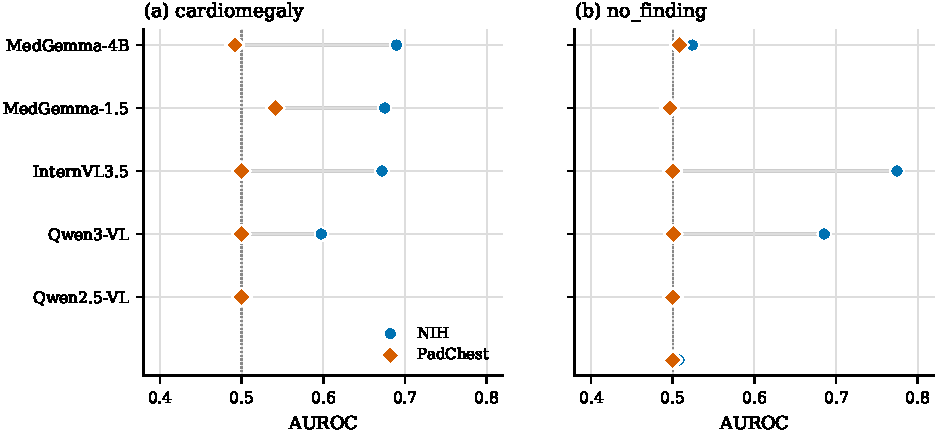
\includegraphics[width=\textwidth]{figures/fig04_transfer.pdf}
\caption{跨数据集迁移（NIH $\rightarrow$ PadChest）。每条线段连接同一模型的 NIH AUROC 与 PadChest AUROC；虚线为随机水平。}
\label{fig:transfer}
\end{figure}

\subsection{报告层：依赖标注器的排序}
\label{sec:results-report}

\begin{table}[t]
\centering
\small
\caption{Open-i 报告层（$n=947$，规则标注器）。}
\label{tab:report}
\begin{tabular}{lrrl}
\toprule
模型 & 漏报 & 幻觉 & 体制 \\
\midrule
CheXagent & \textbf{1,198} & \textbf{113} & 多为``无法判读'' \\
MedGemma-1.5 & 571 & 268 & 保守 \\
Qwen2.5-VL & 302 & 2,128 & 中等漏报、高幻觉 \\
InternVL3.5 & 274 & 2,198 & 同上 \\
MedGemma-4B & 196 & \textbf{3,021} & 低漏报、很高幻觉 \\
Qwen3-VL & \textbf{181} & \textbf{3,508} & 最低漏报、最高幻觉 \\
\bottomrule
\end{tabular}
\end{table}

完整 Open-i 表见附录~\ref{app:protocol} 表~\ref{tab:report}。排序依赖标注器。在规则标注器下，两类错误对六个模型的排序方向相反；在 CheXbert 下（同样 947 例研究），幻觉排序方向保持一致（Spearman 0.71，$n=6$，$p=0.11$），而漏报排序不一致（$-0.49$，$p=0.33$；附录~\ref{app:protocol} 表~\ref{tab:chexbert}）。因此我们不主张普遍的漏报--幻觉权衡：表观权衡是规则标注器的属性，只有幻觉轴稳定到可以作为模型排序报告。

\subsection{选择性预测：没有可用覆盖率}
\label{sec:results-selective}

选择性指标需要模式适配器：矩阵运行器把答案嵌在 \texttt{parsed.findings} 下，而 NIH 依赖文件不带真值，直接把现有选择性预测脚本指向它们会得到零行。本节同时是四个前提的\emph{下游代价}：选择性可信层不可能比它所消费的契约更可识别，其覆盖率在任何风险模型拟合之前就已被契约覆盖所界定。使用适配器后，合规覆盖率在各模型间差异显著：Qwen2.5-VL 100\%、InternVL3.5 99.6\%、MedGemma-1.5 95.2\%、Qwen3-VL 91.7\%、MedGemma-4B 87.9\%、\textbf{CheXagent 18.9\%}。逐单元覆盖普查见附录~\ref{app:protocol} 表~\ref{tab:coverage}。

因此，CheXagent 会依约定产生两个互相矛盾的图像级错误率：跳过无概率标签时为 0.183，把所有非阳性状态视为阴性时为 1.000。两者都不错；它们回答不同问题。它的选择性指标与其他五个不可比，报告时附 \texttt{contract\_coverage} $=0.189$（\texttt{not\_mentioned} $=9{,}486/12{,}016$ 个槽位；只有 9.7\% 的图像八个标签全部确定）。

\begin{table}[t]
\centering
\footnotesize
\setlength{\tabcolsep}{2pt}
\caption{NIH 留出测试集上的选择性预测（$n=1{,}054$ 例研究；8,432 个发现项；427 个患者簇）。``风险''是已回答项中的错误率。AUROC 列为发现级错误检测 AUROC，分别使用单独置信度与置信度加 shift 分数。}
\label{tab:selective}
\begin{tabular}{lrrrrrrr}
\toprule
模型 & 发现错误 & 覆盖@5\% & 覆盖@10\% & 风险@50\% & 风险@80\% & AUC（置信） & +shift \\
\midrule
MedGemma-4B & 0.335 & 0.064 & 0.249 & 0.232 & 0.322 & 0.644 & 0.678 \\
MedGemma-1.5 & 0.323 & 0.093 & 0.332 & 0.173 & 0.270 & 0.737 & 0.737 \\
InternVL3.5 & 0.319 & 0.000 & 0.117 & 0.235 & 0.302 & 0.627 & 0.635 \\
Qwen3-VL & 0.392 & 0.010 & 0.025 & 0.256 & 0.377 & 0.660 & 0.664 \\
Qwen2.5-VL & 0.440 & 0.005 & 0.020 & 0.234 & 0.375 & 0.772 & 0.773 \\
\bottomrule
\end{tabular}
\end{table}

图像级错误被上限主导：每例 NIH 评估研究都至少在一个八标签上为阳性（92\% 至少有一个疾病标签，其余仅为 no-finding），因此全阴预测器的错误率为 0，0.94--0.97 是构成导致的上界伪影。发现级才是可解释的层级（表~\ref{tab:selective}）。在该层级，把 shift 分数加入置信度最多使 AUROC 变化 $+0.034$（MedGemma-4B 0.644$\rightarrow$0.678，InternVL3.5 0.627$\rightarrow$0.635，Qwen3-VL 0.660$\rightarrow$0.664，Qwen2.5-VL 0.772$\rightarrow$0.773），对 MedGemma-1.5 没有影响（0.737$\rightarrow$0.737）；加入图像依赖使两个 MedGemma 模型分别提高 $+0.033$ 与 $+0.006$。因此，排序接近单独置信度已经提供的水平；同时，在 5\% 风险预算下没有模型超过 9.3\% 覆盖率。三动作策略在图像级从不接受（接受率 0.000）。在发现级，它对五个可比模型接受 17--41\% 的条目（CheXagent 在其 18.9\% 契约覆盖下为 12--17\%），但接受项的误差率为 5.7--21.7\%，在每个单元都高于 5\% 预算。因此，它是在唯一能行动的层级上未通过预算，而不是通过拒绝行动来``通过''。

完整风险--覆盖曲线（附录~\ref{app:risk}，图~\ref{fig:risk}）说明 5\% 负结果不是某个阈值的伪影。在 5\% 覆盖率处，风险已达 0.043--0.154；到 10\% 覆盖率时，每个模型都超过 5\% 预算。10\% 预算下的覆盖率为 0.020--0.332；50\% 与 80\% 覆盖率处的风险分别为 0.173--0.256 与 0.270--0.377。该策略在 5\% 下从未达到可用工作点；它在临床认可的 10--20\% 预算下是否可用，是部署决策，而不是本文的主张。

\subsection{受控复现实验}
\label{sec:results-round2}

既有文献留下三个决定上述结论可外推程度的问题：有监督模型是否也会停在随机水平；schema 结果是否只是某一个检查点的习惯；第二个推理模型是否显示同样的轴。本节用预先部署的对照回答这三个问题，并针对 schema 结果检验第四个问题——跨家族的一般性；其余跨家族主张仍未解决，并如实标注。

\subsubsection{监督基线并不处于随机水平}
\label{sec:results-baseline}

我们用 ImageNet 初始化训练 DenseNet-121~\citep{huang2017densely}：$224$\,px、类别加权 BCE、AdamW、固定八个 epoch，不做早停、不做基于测试集的选择。它只见过 3,871 张 \texttt{internal\_train} 图像，与 1,506 例评测研究没有任何患者重叠。在同样的七个病理标签上，它取得\textbf{宏 AUROC 0.733}（95\% 患者聚类自助法区间 0.718--0.749，725 名患者，1,000 次重采样；逐标签 0.620--0.805；表~\ref{tab:baseline}），在其自身 1,352 例患者不重叠的 \texttt{internal\_test} 划分上为 0.724（VLM 评测使用该划分中的 1,054 例子集；第~\ref{sec:protocol} 节）。

\begin{table}[t]
\centering
\small
\caption{干净 NIH 七个病理标签的宏 AUROC（$n=1{,}506$）。基线只用 3,871 张无患者重叠的图像训练；六个 VLM 即表~\ref{tab:clean} 的矩阵。}
\label{tab:baseline}
\begin{tabular}{lrr}
\toprule
模型 & 宏 AUROC & 家族 \\
\midrule
\textbf{DenseNet-121（监督）} & \textbf{0.7329} & CNN，本文训练 \\
MedGemma-4B & 0.6270 & 医学 VLM \\
InternVL3.5-8B & 0.6066 & 通用 VLM \\
MedGemma-1.5 & 0.5852 & 医学 VLM \\
Qwen3-VL-8B & 0.5455 & 通用 VLM \\
Qwen2.5-VL-7B & 0.5013 & 通用 VLM \\
CheXagent-8B & 0.5001 & 胸片专用 \\
\bottomrule
\end{tabular}
\end{table}

因此，这些标签从这些图像上是可学的，水平 0.73，而训练集只有 3,871 张——不到公开训练划分 86,524 张的 5\%。``没有可用判别力''说的是模型，不是任务或单纯的标签噪声。基线也给出反方向的界：0.73 并非临床级，故本文的负结果针对的是\emph{测量可识别性}，而不是胸片分类本身不可能。

\subsubsection{schema 依赖性在第二个医学模型上复现，但映射不同}
\label{sec:results-schema2}

我们在 MedGemma-1.5 上重做五套 schema 扫描（15,060 次调用）。核心结果复现：在空白图像上，\textbf{五套 schema 的病理召回全部为 0.000}，而真实图像上为 0.493--0.614（表~\ref{tab:r2schema}）。没有任何措辞能制造图像依赖。

\emph{未}复现的是每套 schema 落入哪种失效形态。MedGemma-4B 有两种（自信判正常，或被迫弃权）；MedGemma-1.5 出现三种：自信判正常（v0、v1、v3 的空白回答中 \texttt{no\_finding} 阳性率 100\%）、\emph{契约坍缩}（v2 仍给标签但在 99.9\% 的空白回答中丢掉概率对象）、以及拒绝断言（v4 在 100\% 的空白回答中判 \texttt{no\_finding} 阴性，并同样契约坍缩）。真实图像召回最高的是 v4（0.614，比 v0 高 6.3\,\pp{}），而它的空白召回仍为 0.000：提示词移动的是工作点，不是模型获取证据的能力。

正确的表述因此比第~\ref{sec:results-schema} 节的``契约决定捷径的形式''更窄：契约与模型\emph{共同}决定形式，而且这一联合映射不可跨检查点迁移。可迁移的是对基准真正重要的不变性：真实图像召回与空白图像行为由不同因素决定，因此任何 schema 都不能只靠其中之一来验证。

\subsubsection{空白图像结果跨模型家族成立；契约签名不成立}
\label{sec:results-xfamily}

为区分 MedGemma 习惯与契约效应，我们在 Qwen3-VL-8B（不同家族的通用模型）上重做扫描（表~\ref{tab:r2xfamily}）。空白图像结果精确复现：三套 schema 下空白图像的病理召回均为 \textbf{0.000}，真实图像为 0.258--0.306。可观察签名没有复现：Qwen3 的 v0 是自信正常（空白回答中 \texttt{no\_finding} 阳性 100\%），但八个请求概率只给出一个，概率完整度空白 12.5\%、真实 47.1\%；v1 保持同样的自信正常答案，同时把完整度恢复到 100\% 与 95.2\%；v4 拒绝正常断言（空白中 \texttt{no\_finding} 阳性 0\%），并在 98\% 的真实回答中契约坍缩。两个模型出现相同的三种失效形态，但 variant 到形态的映射不同。因此契约覆盖是 schema 的属性，而不是模型的属性；空白图像依赖则同时是二者的属性。

\begin{table}[t]
\centering
\footnotesize
\setlength{\tabcolsep}{3.5pt}
\caption{Qwen3-VL-8B 上的跨家族 schema 扫描（每格 $n=1{,}506$）。三套 schema 下空白图像的病理召回均为 0.000，因此空白依赖不是 MedGemma 的习惯。可观察签名不同：v0 自信正常但只给一个概率，v1 自信正常且契约完整，v4 拒绝正常断言并契约坍缩。}
\label{tab:r2xfamily}
\begin{tabular}{lrrrrrr}
\toprule
方案 & 真实召回 & 空白召回 & 空白 \texttt{no\_finding} 阳性 & 违约（真实/空白） & 完整度（真实/空白） \\
\midrule
v0 简单 & 0.306 & \textbf{0.000} & 1.000 & 0.611 / 1.000 & 0.471 / 0.125 \\
v1 逐标签二分类 & 0.258 & \textbf{0.000} & 1.000 & 0.054 / 0.000 & 0.952 / 1.000 \\
v4 正常性施压 & 0.263 & \textbf{0.000} & 0.000 & 0.983 / 1.000 & 0.849 / 0.875 \\
\bottomrule
\end{tabular}
\end{table}

\subsubsection{措辞不是机制，但它决定空白图像上的答案}
\label{sec:results-paraphrase}

我们在 MedGemma-4B 上对 v0 契约做了两个改写版本（标签集合、状态规则、JSON 结构完全一致），对真实与空白图像各跑一遍（6,024 次调用）。真实图像上，发现级答案可复现：与 v0 基线的一致率为 90.9\% 与 91.4\%，Cohen's $\kappa$ 为 0.624 与 0.642。schema 结论不是单一措辞的产物。

空白图像上，两个改写版本与基线只在一个标签上分歧。v0 在 100\% 的空白回答中判 \texttt{no\_finding} 阳性；p2 相同（一致率 1.000）；p1 在 100\% 中判阴性（一致率 0.000）。病理标签在三者之间完全一致（全阴性，一致率 1.000）。也就是说，空白图像上的答案由措辞决定、不含任何图像信息——这正是为什么零模型前提需要一个空白对照\emph{并且}一个措辞对照，而不是二者之一。

该对照也在 Qwen3-VL 上运行（表~\ref{tab:r2para}）。两个改写版本都复现真实图像答案（p1 一致率 93.1\%，$\kappa$ 0.723；p2 90.3\%，$\kappa$ 0.701），但都不翻转空白图像答案：与 v0 的空白一致率均为 1.000，而 p1 会把 MedGemma-4B 的空白答案完全翻转。因此措辞设定的是模型特定的先验：同一改写把 MedGemma 的空白答案变负，却让 Qwen3 的自信正常答案保持不变。

\subsubsection{第二个推理模型：同一工作点，新的失效模式}
\label{sec:results-second}

Qwen3-VL-8B-Thinking 具有原生推理通道（chat 模板预填 \texttt{<think>}，模型在回答前闭合它），因此可察觉性轴第一次能在第二个模型上读出。我们在全部 1,506 例研究上跑了七个格子（clean 加六个 severe）。只有闭合推理块\emph{并且}其后能解析出 JSON 的回复才算可用答案，其余作为实测结果保留（表~\ref{tab:r2recon}）。

\textbf{覆盖率本身是可测量，且随退化下降。} 在 5,120 token 预算下，10,542 个格子中有 9,381 个给出可用答案（89.0\%）；对 40 个格子的 8,192 token 抽样再补 20 个（最终 89.2\%）。覆盖率为 clean 92.6\%、分辨率 severe 80.9\%、亮度 severe 84.3\%（表~\ref{tab:r2think}）。失败并非``加大预算即可消除的截断''：仍然失败的回复中位长度在 2,560 上限时为 9.8k 字符、3,584 时为 13.5k、5,120 时为 19.3k，在 8,192 的 40 格随机抽样中为 28.1k——它们会撑满给它的任何预算；8,192 抽样只能救回 50\%（表~\ref{tab:r2budget}）。不终止是模型行为，我们按行为报告。这是 overthinking 文献在视觉语言模型上的对应：超过某个点，追加推理 token 的边际价值为负，并可能放弃模型本来已经得到的答案~\citep{wu2026whenmore,zhou2026overthinking}；被截断的推理链可能比不推理更糟~\citep{su2026broken}。这里的失效更严重——回复根本无法解析——因此预算曲线是该模型的测量属性，而不只是成本。

\begin{table}[t]
\centering
\footnotesize
\setlength{\tabcolsep}{3.5pt}
\caption{第二个推理模型，severe 格（每格 $n=1{,}506$）。覆盖率为 5,120 token 预算下给出可用答案的研究比例；$\Delta$ 召回为与 clean 在同一批共同作答研究上的配对差（noise $n=1{,}238$；resolution $n=1{,}132$）。AUROC 为七个病理标签的宏平均；阳性率为被判阳性的病理槽位比例。}
\label{tab:r2think}
\begin{tabular}{lrrrrr}
\toprule
格子 & 覆盖率 & 链长(k) & 阳性率 & 宏 AUROC & $\Delta$ 召回 \\
\midrule
clean & 0.926 & 8.73 & 0.250 & 0.547 & --- \\
blur & 0.932 & 8.84 & 0.189 & 0.547 & $-5.5$\,\pp{} \\
brightness & 0.843 & 9.56 & 0.213 & 0.550 & $-5.1$\,\pp{} \\
contrast & 0.924 & 8.99 & 0.280 & 0.545 & $+2.2$\,\pp{} \\
JPEG & 0.923 & 9.37 & 0.240 & 0.537 & $-1.8$\,\pp{} \\
noise & 0.885 & 9.06 & 0.173 & 0.527 & $\mathbf{-10.3}$\,\pp{} \\
resolution & \textbf{0.809} & \textbf{10.22} & \textbf{0.125} & 0.549 & $\mathbf{-13.2}$\,\pp{} \\
\bottomrule
\end{tabular}
\end{table}

\textbf{工作点机制复现，方向相反。} 分辨率损失下阳性率由 0.250 降至 0.125，\texttt{no\_finding} 阳性率由 0.283 升至 0.450，而宏 AUROC 在各格中稳定在 0.527--0.550。由于覆盖率同时下降，我们在配对子集（两格都给出可用答案的研究）上重算该比率：0.250 $\rightarrow$ 0.128，即这一移动不是覆盖率伪影（附录~\ref{app:round2}，表~\ref{tab:r2posrate}）。模型并未丢失排序信息——它本来就没有——它把工作点移向``正常''。这与第~\ref{sec:results-op} 节互为镜像：那里干净阳性率高的模型在退化下上移、召回上升；这里干净阳性率仅 25\% 的模型下移、召回下降。二者都是工作点移动，都不是鲁棒性变化。

逐标签看，配对损失经聚类自助法与多重比较控制后依然显著：胸腔积液 $-8.8$ $[-11.9,-5.8]$\,\pp{}、肺炎 $-11.0$ $[-16.4,-5.5]$\,\pp{}（$q<0.001$）、心影增大 $-6.0$ $[-9.9,-1.9]$\,\pp{}（$q=0.014$）、肺不张 $-2.2$ 与肺水肿 $-4.2$\,\pp{}（$q=0.053$），实变与气胸不显著（表~\ref{tab:r2label}）。

\textbf{轴对通用，象限不通用。} 以覆盖率损失作为该模型的可察觉性读数、以配对召回变化作为损伤，两者再次可分离（与 $|\Delta|$ 的 Spearman 0.49，$p=0.33$；与带符号 $\Delta$ 的为 $-0.54$，$p=0.27$；$n=6$）。在同一 $|\Delta|$ 定义下，MedGemma-1.5 的标记--损伤相关也是 0.49，但六个点使两个估计都无法与零区分：我们主张同一\emph{方向}，而不是共同斜率。噪声换位了：对 MedGemma-1.5，噪声是静默退化（标记率 0.46\%，倒数第二低）而损伤与分辨率损失相当；对 Qwen3-VL-Thinking，噪声是响亮的（覆盖率损失 11.5\%，第三高），并造成 10.3\,\pp{} 的召回损失。\emph{静默失效是监测通道的属性，而不是退化的属性}：盯着推理是否终止的通道能看见噪声，盯着某个特定标记词的通道看不见。

这也解释了为什么第二个模型没有复现反转 3 的正号。该反转需要阳性率有上行空间；一个只把 25\% 槽位判阳的模型几乎没有空间，退化只能把它往下推。按第四前提报告工作点，正是使两个模型可比的原因。


\subsection{核心判断的敏感性}
\label{sec:sensitivity}

三个最关键阈值已在全范围扫描（附录~\ref{app:risk}，\url{scripts/81_sensitivity_analyses.py}）。19 格网格本身是探索性的剂量--响应设计：逐格对照是描述性的，未跨格子做多重比较校正，也不对其附加族错误率主张。确证性的量是第~\ref{sec:preconditions}~节声明的四个审计统计量，以及第~\ref{sec:results-round2} 节的复现实验。

\textbf{(i) 坍缩规则。}把众数占比阈值在 $0.30$--$0.80$ 上变化、唯一回答数上限在 $1$--$20$ 上变化，只会改变哪些边际单元被标记（表~\ref{tab:sweep}），不改变跨数据集结论：在 PadChest 上，六个模型中有五个在 $0.40$ 至 $0.80$ 的每个阈值下都坍缩；在最宽松的 $0.30$ 切点，给出 329 种不同回答的 MedGemma-1.5 也被标记，因此六个全部坍缩。域内被标记集合随阈值升高而缩小（Qwen3-VL 在 $0.60$ 退出，CheXagent 在 $0.70$ 退出）；在 Open-i 上，MedGemma-4B 在低于 $0.70$ 时被标记，$0.30$ 时 Qwen3-VL 也被标记。本文没有任何主张依赖这些边际单元。

\textbf{(ii) 真实图像间零模型的配对。}对 Open-i，在 (a) 随机图像对与 (b) 参考报告长度匹配对下重算真实图像间 Jaccard。零模型最多变化 $0.020$（表~\ref{tab:sens}；MedGemma-4B：0.824 对 0.844），所有分离保持符号与量级：Qwen3-VL 仍远高于其零模型（$+0.648$ 对 $+0.643$），Qwen2.5-VL 保持 $+0.19$，MedGemma-4B 与 MedGemma-1.5 保持负值（$-0.070$ 与 $-0.087$）。``空白是另一种模板，而不是证据''这一解读对配对规则稳健。

\textbf{(iii) 多重比较校正下的迁移区间。}表~\ref{tab:transfer} 报告的跨数据集 $\Delta$AUROC 区间是单次两两 95\% 区间。我们对该家族的 16 个可估计模型--标签单元做 Bonferroni 校正（$z=2.955$）。四个大损失全部存活：InternVL3.5 \texttt{cardiomegaly}（校正后上界 $-0.127$）、InternVL3.5 \texttt{consolidation}（$-0.048$）、MedGemma-4B \texttt{cardiomegaly}（$-0.136$）、MedGemma-1.5 \texttt{cardiomegaly}（$-0.030$）仍严格低于零。两个边缘差值（MedGemma-4B 与 MedGemma-1.5 的 \texttt{no\_finding}）变为不显著，一些本来就接近随机的实变与心脏增大小单元也是如此；四个大损失不受影响。``迁移坍缩''这一主张稳健；少数接近零的单元则不是。

\textbf{(iv) 工作点构成。}InternVL3.5 对比度/重度单元在单张图像层面分解（附录~\ref{app:risk}）。在转移最多的三个发现中，``召回增益''完全来自干净条件下为阴性的图像上的新真阳性（$gt\_pos$：分别获得 $+43$、$+30$、$+50$，丢失 $10$、$3$、$1$），而此前正确的阴性状态以相当的比例翻转为假阳性（$gt\_neg$：$+36$、$+59$、$+69$）。净假阳性上升（表~\ref{tab:op}）。这与广泛的工作点移动一致，而不是有针对性地找回丢失发现；它本身不能识别阈值机制。

\begin{figure}[t]
\centering
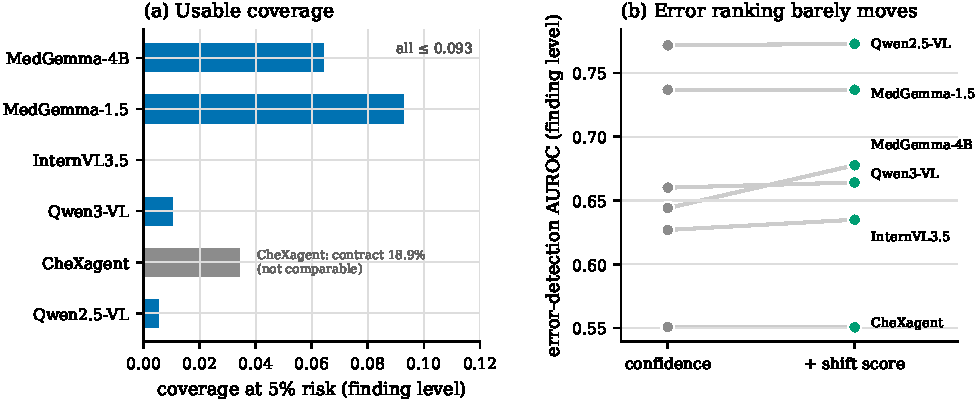
\includegraphics[width=\textwidth]{figures/fig06_selective.pdf}
\caption{(a) 5\% 风险预算下的可用覆盖率最多为 0.093；CheXagent 的柱为灰色，因为其契约只覆盖 18.9\% 的槽位。(b) 在发现级，同样的信号只使错误排序发生边际变化。排序能力与决策有用性是两件事。}
\label{fig:selective}
\end{figure}

\begin{figure}[t]
\centering
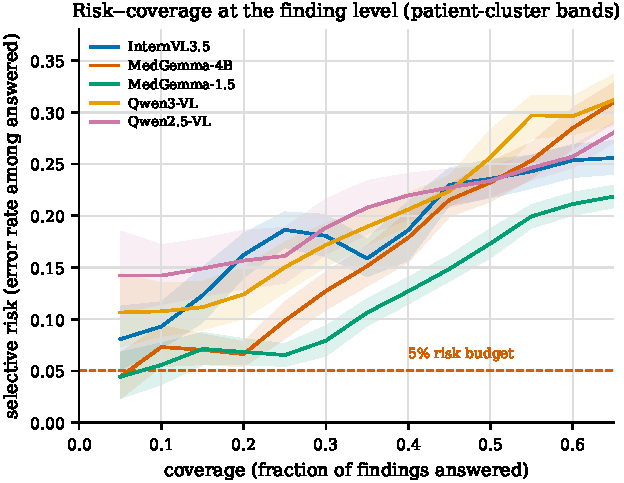
\includegraphics[width=0.62\textwidth]{figures/fig07_risk_coverage.pdf}
\caption{发现级风险--覆盖曲线，含患者聚类自助法带（1,000 次重采样）。在 5\% 覆盖率处风险为 0.043--0.154；到 10\% 覆盖率时每个模型都超过 5\% 预算；5\% 预算最多允许 0.093 覆盖率，10\% 预算允许 0.02--0.33，具体取决于模型。}
\label{fig:risk}
\end{figure}

\section{讨论}
\label{sec:discussion}

\textbf{四次反转的共同结构。}每一个都是分母从未被建立的比值：没有零模型的对照、没有阳性预测率的召回率、分母未知的分数、跨两种输出体制的比较。修复是程序性的，而不是架构性的。四项审计都可以在 CPU 上、对基准本来就已写出的工件运行，只需几分钟。

\textbf{一份报告清单。}我们建议，任何形如``模型 $M$ 依赖图像''、``模型 $M$ 鲁棒''或``$M$ 可迁移''的主张都应附带：(1) 真实条件下的输出支撑大小与众数占比；(2) 对照的真实图像间零模型；(3) 阳性召回率、阳性预测率与精确率；(4) 契约覆盖与输出模式指示量；(5) 有效输入分辨率与精度；(6) 每个指标的分母。前四项是前提，后两项是测量声明。

\textbf{为什么文献需要重读。}此前的无图像消融报告对照，却没有零模型，也没有输出支撑检查。我们的结果表明，这些数字至少有两种误导方式：拒答模板产生很大的对照却没有证据提取；坍缩模型因为缺乏变化而产生零对照。这不是对任何具体论文执行的批评；而是在说，按常见方式计算的统计量并不能识别目标量。

\textbf{静默失效是与部署最相关的象限。}如果监控系统监视不确定性、拒答或推理通道激活，它能抓住分辨率损失与模糊，却会漏掉噪声。这种不对称不是某个模型的性质：五个模型的合并标记率在分辨率下为 14.40\%，在噪声下为 0.093\%，而召回损伤相当。我们谨慎界定它说明与不说明什么。标记率是\emph{模型侧}信号，不是人类或图像侧可见性的度量；在同一批数据上，一个无参考 Laplacian 方差统计量以 AUC $1.000$ 区分干净与重度噪声，基于规则的搜索在任何重度噪声回答中都找不到显式质量语言（附录~\ref{app:risk}，表~\ref{tab:imageside}，以及 \url{scripts/83_quality_language_audit.py}）。因此，主张更窄，也更有用：\emph{模型自身的监控与报告信号检测不到一种已被证明会损害其答案的退化}。实际监控器应把图像侧退化检测器与模型侧犹豫信号结合起来，因为两者在退化谱的两端失效。

\textbf{契约是模型可观测行为的一部分。}模式消融表明，同一组权重可以因所请求的输出契约而成为``自信正常''的捷径，或成为弃答模型。这既是测量警告（契约是一个变量），也是设计杠杆（若希望弃答，可以请求弃答）。它还意味着``模型对空白图像过度自信''不是一个模型级事实。

\textbf{我们未能建立的东西。}激发本研究的 selective-trust 框架未获验证：其组件只使错误排序发生边际变化，且不产生覆盖率。我们把它作为负结果报告，而不是在看到测试集后拟合一个更宽松的阈值。

\section*{局限性}
\label{sec:limitations}

\begin{enumerate}[leftmargin=1.2em,itemsep=2pt,topsep=2pt]
\item \textbf{合成退化。}19 格网格是参数化的，而非真实采集退化。它提供剂量--响应控制，但不复现扫描仪特有的物理过程。
\item \textbf{标签来源。}NIH 标签由报告经 NLP 导出；PadChest 使用 120 标签词表并映射到八种发现，肺炎结构性缺失。标签噪声限制本文每个 AUROC 的上界。共同标签分析（附录~\ref{app:risk}）在两个数据集都标注的七个标签上重算迁移损失；排除肺炎不改变结论。
\item \textbf{跨数据集聚因。}NIH 与 PadChest 同时存在医院来源、病例构成、标签映射与输入几何的差异。共同标签分析去掉了结构性缺失的肺炎项，响应性检查去掉了常数输出解释，但这里没有任何设计能把医院偏移与病例构成偏移分开。我们主张数据集层面的判别力坍缩，而不是量化的医院域惩罚。
\item \textbf{六个模型、一块 GPU、一套解码协议。}贪婪解码最大化可复现性，但可能低估基于采样的部署所具有的输出多样性。
\item \textbf{贪婪解码不具 batch 不变性。}同一 100 张图像在固定种子下用 batch 1、4、8 重跑，有 12--13\% 的图像原始回复发生变化；解析后的状态平均在八个标签中一致 7.96--7.97 个，解析率保持 1.000。该差异比本文报告的退化效应小一个数量级，但我们不主张逐位可复现。
\item \textbf{跨家族输入几何因架构而异}（同一张图像上 0.20--15.24\,MP），无法在不改变模型的情况下拉平。我们报告它而不是隐藏它（表~\ref{tab:geometry}）；受控的输入分辨率扫描需要重跑每个模型，本文未做。
\item \textbf{没有第四个数据集。}该框架在三个数据层上展示；在独立医院或未见模型家族上的外部验证仍是未来工作。
\item \textbf{CheXagent 的契约不是同一任务。}其 79\% 的 \texttt{not\_mentioned} 率使其选择性指标不可比；我们把它排除在比较性选择性主张之外。
\item \textbf{Open-i 打分使用规则标注器，并用 CheXbert 交叉核验。}两种标注器在绝对计数与漏报排序上不一致（Spearman $-0.49$）；幻觉排序方向保持一致（$0.71$）。因此我们只把幻觉排序作为稳定结果报告，不主张普遍的漏报--幻觉权衡。
\item \textbf{监督基线的范围。}基线是单个 DenseNet-121，只用仓库内 3,871 张训练图像训练，而非完整的 11.2 万张 ChestX-ray14，因此 0.733 是这些标签所能支撑性能的下界。它足以区分``任务不可能''与``模型弱''（本文的主张），但不是临床级参照。
\item \textbf{第二个推理模型：覆盖率与预算。}Qwen3-VL-Thinking 网格在 5,120 token 预算下对 10,542 个格子中的 9,381 个给出可用答案（89.0\%），对残余做 8,192 token 抽样后为 9,401 个（89.2\%）；余下 1,141 条不终止，8,192 的 40 格抽样只能救回其中一半，而单次调用成本约翻倍。我们把不终止作为实测结果，并在共同作答的研究上报告配对召回，但逐格的非配对召回会偏向模型``愿意完成''的研究。推理链未经人工核验；我们只主张其长度与终止情况，不主张其忠实性。
\item \textbf{复现实验的覆盖范围。}schema 扫描覆盖第二个医学模型与跨家族模型（Qwen3-VL），改写对照覆盖两个模型；双轴结果仍建立在两个具有不同通道的模型上，比单模型强，但仍不是跨家族规律。CheXbert 交叉核验是标注器复现，而不是人工裁决的金标准。
\item \textbf{没有临床结局。}本文不测量诊断获益或伤害。
\item \textbf{LLaVA-Med 是实测排除。}它在 PadChest、Open-i 与一个 200 例 NIH 子集上运行，只产生两个模板且没有发现级内容（NIH 上众数占 98.7\%、结构化解析率 0\%）；它被排除在发现指标之外，但没有被排除在记录之外。Open-i 没有确定标签，因此我们无法检验它那二值的``不可判读/正常''门控是否与参考报告一致。
\item \textbf{探索性与确认性。}四次反转是带预先声明规则的描述性分析，不是预注册假设检验。所有 18 个数据层--模型单元都被报告，而不是挑选子集；迁移差值额外做了 16 单元 Bonferroni 放宽；其他处不声称 $p$ 值族错误率。
\end{enumerate}

\section*{结论}
\label{sec:conclusion}

这个领域已经习惯把鲁棒性、依赖与迁移报告为模型属性。我们的数据表明，它们是模型--测量系统的属性。四项廉价检查——响应性、同空间零模型、工作点与契约覆盖——在我们研究的三个数据层中都反转了头条结论。两项发现经受住了检查：退化具有两个可分离的描述轴；标签级敏感性层级在 NIH 原始秩上具有模型不变性，但部分受患病率混杂，仍需外部复现。四项确证性实验深化了这两项发现，而不只是重复它们：宏 AUROC 0.733 的监督基线表明``随机水平判别力''是模型属性，且同一 CNN 在固定规则下复现了对比度诱发的工作点移动，因此该反转不是视觉语言模型特有的；schema 扫描与改写对照表明，契约与措辞共同决定模型对``没有证据的图像''说什么；第二个推理模型复现了工作点机制，同时\emph{移动}了静默象限——噪声对 MedGemma-1.5 的标记通道不可见，对``推理是否终止''这一通道却清晰可见。因此，静默失效属于监测器，而不属于退化——这正是本文论点的实践形态。我们原本要验证的选择性可信框架未能成立：其组件只使错误排序发生边际变化，且在 5\% 风险预算下不产生可用覆盖率（最多覆盖 9.3\% 的发现）。

建设性的主张是谦逊的，我们认为也比排行榜更有用：在报告数字之前，先报告分母。表~\ref{tab:checklist} 把四个前提变成一份清单，任何基准都可以把它套用到已有的预测文件上。

\begin{table}[h]
\centering
\small
\caption{面向图像依赖、鲁棒性与迁移主张的最小报告清单。每一行都可以在冻结的预测文件上评估，无需重跑模型。}
\label{tab:checklist}
\begin{tabular}{p{0.17\textwidth}p{0.34\textwidth}p{0.34\textwidth}}
\toprule
前提 & 报告 & 判为失败的条件 \\
\midrule
P1 响应性 & 真实输入上的唯一归一化回答数与众数占比（带区间）；空白模板占比 & 众数占比 $\ge 0.50$ 或唯一回答数 $\le 5$：无可测响应，而非``零依赖'' \\
P2 零模型 & 相对真实-真实零模型的同空间分离 $\Delta_{\text{null}}$；写明度量与其极性 & $\Delta_{\text{null}} \approx 0$：该对照是自然变异或样板文本 \\
P3 工作点 & 在已声明规则下的召回率\emph{与}阳性预测率、精确率及病例级转移 & 召回变化而阳性率未报告：阈值移动与鲁棒性无法区分 \\
P4 契约覆盖 & 确定槽位占比、状态分布、输出模式（推理标记、概率完整度） & 被比较单元的分母或输出体制不同：数字不在同一尺度上 \\
\midrule
推理附加项 & 在已声明 token 预算下的终止率，以及预算曲线 & 各单元覆盖率不同：在共同作答研究上配对报告条件指标 \\
\bottomrule
\end{tabular}
\end{table}

\section*{可复现性}

所有工件随稿发布。响应性审计与选择输入适配器是纯 CPU 脚本；每张图都由冻结的预测文件生成，而不是从转录数字生成。主运行状态（38 个阶段条目：30 个已完成，其中 8 个在结构化契约指标上标记为契约豁免——六个 Open-i 阶段与两个 LLaVA 阶段；Open-i 的散文指标仍然计分）记录在可恢复的状态文件中；预处理契约——包括每个模型的有效输入几何——单独记录。全口径调用总数为 275,618：六模型矩阵 270,324，LLaVA-Med 5,294（PadChest 3,000、Open-i 1,894、NIH 子集 400）。环境清单记录了三个模型专用环境：\texttt{.venv-vl}（Python 3.10，torch 2.5.1+cu121，transformers 4.51.3）用于 MedGemma、Qwen2.5-VL 与 InternVL；\texttt{.venv-chexagent}（torch 2.1.0）用于 CheXagent；\texttt{.venv-modern}（torch 2.14.1+cu126，transformers 5.18.0）用于 Qwen3-VL。冻结依赖锁位于 \texttt{program/env/lock-*.txt}。脚本 75--101 生成 CSV 工件；图由脚本 80 生成；正文表格由脚本 104 逐项对照这些 CSV 校验。41 阶段覆盖普查报告 284,695 次已交付调用：270,324 次六模型矩阵、9,477 次第二推理模型（9,401 个可用单元加 76 次冒烟调用）、4,894 次 LLaVA-Med 的 PadChest 与 Open-i 调用；400 例 LLaVA-Med NIH 子集在 41 个已交付阶段之外，因此与全口径总数恰好相差 9,077 次。附有只含计分行的 \texttt{nih\_eval\_1506.csv}（1,506 行，SHA-256 记录于 \texttt{MANIFEST\_SHA256.json}），使计分集及其分母可审计。纯 CPU 的崩溃/恢复测试（40 项检查，桩模型）与 \texttt{cxr\_trust} 单元测试无需 GPU 即可运行。数据许可仍归原始发布方（NIH ChestX-ray14、PadChest、Open-i），模型检查点按其上游许可使用。


\FloatBarrier
\bibliographystyle{unsrtnat}
\bibliography{refs}

\appendix
\section{工件索引}
\label{app:artifacts}

\begin{table}[H]
\centering
\footnotesize
\setlength{\tabcolsep}{4pt}
\renewcommand{\arraystretch}{0.92}
\caption{支撑本文每个数字的工件。}
\label{tab:artifacts}
\begin{tabular}{ll}
\toprule
项目 & 路径 \\
\midrule
响应性审计 & \url{scripts/78_responsiveness_audit.py} \\
选择输入适配器 & \url{scripts/79_export_selective_inputs.py} \\
绘图脚本 & \url{scripts/80_make_figures.py} \\
敏感性分析 & \url{scripts/81_sensitivity_analyses.py} \\
图像侧可检测性 & \url{scripts/82_image_side_baseline.py} \\
质量语言审计 & \url{scripts/83_quality_language_audit.py} \\
PadChest 疾病阳性子集 & \url{scripts/84_padchest_abnormal_subset.py} \\
工作点区间 & \url{scripts/85_operating_point_ci.py} \\
患病率分层 & \url{scripts/87_label_hierarchy_prevalence.py} \\
逐标签 CI / BH-FDR & \url{scripts/88_per_label_ci_fdr.py} \\
固定阈值事后分析 & \url{scripts/89_fixed_threshold_posthoc.py} \\
覆盖普查 & \url{scripts/90_coverage_census.py} \\
清单锁定 & \url{scripts/91_manifest_lock.py} \\
round-2 汇总 & \url{scripts/96_analyze_round2.py} \\
配对阳性率 & \url{scripts/102_paired_positive_rate.py} \\
DenseNet 患者自助法 & \url{scripts/103_densenet_bootstrap.py} \\
表格一致性核查 & \url{scripts/104_table_consistency_check.py} \\
输出清单 & \url{scripts/105_outputs_manifest.py} \\
干净 AUROC 区间 & \url{scripts/106_clean_auroc_ci.py} \\
PadChest 标签层级 & \url{scripts/107_padchest_label_hierarchy.py} \\
固定规则重跑 & \url{scripts/108_fixed_rule_rerun.py} \\
CheXbert 交叉核验 & \url{scripts/109_chexbert_openi.py} \\
贪婪确定性 & \url{scripts/110_compare_determinism.py} \\
DenseNet 19 格网格 & \url{scripts/111_densenet_grid.py} \\
跨家族 schema & \url{scripts/112_analyze_xfamily_schema.py} \\
DenseNet 条件指标 & \url{scripts/113_densenet_conditions.py} \\
标注器一致性 & \url{scripts/114_report_labeller_agreement.py} \\
LLaVA-Med NIH 子集 & \url{scripts/115_llava_nih.py} \\
跨家族改写 & \url{scripts/116_paraphrase_xfamily.py} \\
确定性输出 & \url{outputs/determinism/medgemma_4b_it/determinism.csv} \\
固定规则输出 & \url{outputs/fixed_rule/} \\
LLaVA-Med NIH 运行 & \url{outputs/llava_nih/} \\
敏感性结果表 & \url{outputs/analysis_sensitivity/} \\
响应性结果表 & \url{outputs/analysis_responsiveness/} \\
LLaVA-Med 响应性 & \url{outputs/analysis_responsiveness_llava/} \\
契约覆盖 & \url{outputs/analysis_selective/export_manifest.json} \\
地理迁移汇总 & \url{outputs/geographic/<model>/} \\
选择性指标 & \url{outputs/selective_v2/}, \url{outputs/trust_v1/} \\
风险--覆盖带 & \url{outputs/selective_v2/<model>/risk_coverage_bands.csv} \\
跨参数挖掘 & \url{outputs/analysis_nih_mine/joint_*.csv} \\
运行状态（38 阶段） & \url{outputs/state/run_all_layers_state.json} \\
预处理契约 & \url{docs/55_preprocessing_contract.md} \\
\bottomrule
\end{tabular}
\end{table}

\section{协议表}
\label{app:protocol}

\begin{table}[H]
\centering
\small
\caption{NIH shift 网格上的解析与契约覆盖（每模型 28,614 次调用）。``全部确定''是解析成功回答中八个状态全为阳性/阴性的比例。完整 41 阶段普查（交付的 39 个阶段加两个 round-2 推理阶段）见 \url{outputs/analysis_sensitivity/coverage_census.csv}。}
\label{tab:coverage}
\begin{tabular}{lrrr}
\toprule
模型 & 解析率 & 全部确定 & 错误行 \\
\midrule
Qwen2.5-VL & 1.000 & \textbf{1.000} & 0 \\
InternVL3.5 & 1.000 & 0.956 & 0 \\
MedGemma-1.5 & 0.998 & 0.824 & 0 \\
Qwen3-VL & 1.000 & 0.795 & 0 \\
MedGemma-4B & 1.000 & 0.605 & 0 \\
CheXagent & 0.985 & \textbf{0.096} & 0 \\
\bottomrule
\end{tabular}
\end{table}

\begin{table}[H]
\centering
\small
\caption{同一批 947 例 Open-i 研究在两种标注器下的结果（均为槽位级：八个标签 $\times$ 947 次判定）。绝对计数不可跨标注器比较，但排序可以。幻觉排序方向保持一致（Spearman 0.71，$n=6$，$p=0.11$），漏报排序不一致（$-0.49$，$p=0.33$）。}
\label{tab:chexbert}
\begin{tabular}{lrrrr}
\toprule
模型 & 规则漏报 & 规则幻觉 & CheXbert 漏报 & CheXbert 幻觉 \\
\midrule
MedGemma-4B & 196 & \textbf{3,021} & 118 & 609 \\
MedGemma-1.5 & 571 & 268 & 103 & 583 \\
InternVL3.5 & 274 & 2,198 & 187 & 870 \\
Qwen3-VL & \textbf{181} & \textbf{3,508} & 363 & 786 \\
Qwen2.5-VL & 302 & 2,128 & 231 & 660 \\
CheXagent & \textbf{1,198} & \textbf{113} & 165 & 532 \\
\bottomrule
\end{tabular}
\end{table}

\section{有效输入几何}
\label{app:geometry}

\begin{table}[H]
\centering
\small
\caption{最大 PadChest 图像（15.37\,MP）上的有效输入几何。同一张胸片变成六种不同输入；这是测量声明，不是中性设置。}
\label{tab:geometry}
\begin{tabular}{llrl}
\toprule
模型 & 有效输入 & 图像 token 数 & 缩放机制 \\
\midrule
Qwen3-VL-8B & 15.24\,MP & 14,884 & 契约提示 \\
Qwen2.5-VL-7B & 12.85\,MP（上限） & 16,384 & 检查点配置 \\
MedGemma-4B/1.5 & 0.80\,MP & 256 & 固定处理器 \\
InternVL3.5-8B & 0.20\,MP & 256 & $1\times1$ 切片网格 \\
CheXagent-8B & 0.20\,MP & 0（交叉注意力） & 固定处理器 \\
LLaVA-Med-7B & 0.11\,MP & 576 & 固定 CLIP \\
\bottomrule
\end{tabular}
\end{table}

\section{敏感性分析}
\label{app:risk}

所有数值由脚本 81--85（表~\ref{tab:artifacts}）从冻结预测文件与原始图像生成。

\begin{table}[H]
\centering
\small
\caption{众数占比阈值扫描下的坍缩标记（唯一回答数上限固定为 5）。跨数据集判定在 0.40 以上不变；只有在最宽松的 0.30 切点，PadChest 的第六个模型才加入，且只有域内与散文单元在边际上移动。}
\label{tab:sweep}
\begin{tabular}{lrrrrrr}
\toprule
数据层 & 0.30 & 0.40 & 0.50 & 0.60 & 0.70 & 0.80 \\
\midrule
NIH（共 6） & 3 & 3 & 3 & 2 & 1 & 1 \\
PadChest（共 6） & 6 & 5 & 5 & 5 & 5 & 5 \\
Open-i（共 6） & 2 & 1 & 1 & 1 & 0 & 0 \\
\bottomrule
\end{tabular}
\end{table}

\begin{table}[H]
\centering
\footnotesize
\setlength{\tabcolsep}{3pt}
\caption{两个跨域统计量的敏感性。共同标签 $\Delta$AUROC 排除肺炎（在 PadChest 中结构性缺失）。零模型在随机真实图像对与参考长度匹配真实图像对下重算。CheXagent 只有一个可估计的共同标签（记为``(1)''）。最后一列是两种零模型下 $\Delta_{\text{null}}$ 的范围；正值表示空白干预比随机真实图像离真实图像更远。}
\label{tab:sens}
\begin{tabular}{lrrrrrr}
\toprule
模型 & 平均 $\Delta$（7 标签） & 最差标签 & $J$(真实,空白) & 零模型（随机） & 零模型（长度） & $\Delta_{\text{null}}$ 范围 \\
\midrule
MedGemma-4B & $-0.107$ & $-0.246$ & 0.894 & 0.824 & 0.844 & $-0.070$ 至 $-0.050$ \\
MedGemma-1.5 & $-0.079$ & $-0.161$ & 0.736 & 0.648 & 0.654 & $-0.087$ 至 $-0.081$ \\
InternVL3.5 & $-0.134$ & $-0.274$ & 0.562 & 0.673 & 0.677 & $+0.112$ 至 $+0.116$ \\
Qwen3-VL & $-0.059$ & $-0.185$ & 0.091 & 0.740 & 0.734 & $+0.643$ 至 $+0.648$ \\
CheXagent & $-0.004$ (1) & $-0.004$ & 0.277 & 0.247 & 0.252 & $-0.030$ 至 $-0.024$ \\
Qwen2.5-VL & $-0.002$ & $-0.008$ & 0.576 & 0.770 & 0.767 & $+0.191$ 至 $+0.193$ \\
\bottomrule
\end{tabular}
\end{table}

\begin{table}[H]
\centering
\footnotesize
\setlength{\tabcolsep}{3pt}
\caption{标签层级部分受患病率混杂。A 面板：每个模型的保持率与 NIH 患病率 Spearman，以及高/低患病率标签分层的平均保持率。B 面板：秩残差化患病率前后的两两一致性。原始一致性为正，但偏一致性在不同模型对间变号，因此我们不主张患病率无关的病灶规律。}
\label{tab:hierarchy}
\begin{tabular}{lrrr}
\toprule
\multicolumn{4}{l}{\emph{A 面板：保持率与患病率}} \\
模型 & $\rho$(保持率, 患病率) & 平均保持率（高患病率） & 平均保持率（低患病率） \\
\midrule
InternVL3.5 & 0.571 & 0.935 & 0.764 \\
Qwen3-VL & 0.429 & 0.718 & 0.629 \\
MedGemma-1.5 & 0.714 & 0.873 & 0.701 \\
MedGemma-4B & 0.464 & 0.735 & 0.514 \\
\midrule
\multicolumn{4}{l}{\emph{B 面板：模型对一致性}} \\
模型对 & 原始 $\rho$ & 偏 $\rho$ & 精确 $p$ \\
\midrule
InternVL / Qwen3 & 0.771 & 0.765 & 0.658 \\
InternVL / MedGemma-1.5 & 0.857 & $-0.654$ & 0.012 \\
InternVL / MedGemma-4B & 0.750 & $-0.685$ & 0.200 \\
Qwen3 / MedGemma-1.5 & 0.657 & 0.525 & 0.058 \\
Qwen3 / MedGemma-4B & 0.657 & $-0.691$ & 0.242 \\
MedGemma-1.5 / MedGemma-4B & 0.750 & 0.847 & 0.200 \\
\bottomrule
\end{tabular}
\end{table}

\begin{table}[H]
\centering
\footnotesize
\setlength{\tabcolsep}{3pt}
\caption{逐标签干净 $\rightarrow$ 重度召回变化，附患者聚类自助法区间（1,000 次重采样）与每个模型内七个标签的 Benjamini--Hochberg $q$。重度单元合并六种退化类型。心脏增大与接近零召回的气胸是不显著例外；28 个单元中 22 个 $q<0.05$。完整 CSV：\url{outputs/analysis_sensitivity/per_label_bootstrap_fdr.csv}。}
\label{tab:perlabel}
\begin{tabular}{llrrr}
\toprule
模型 & 标签 & $\Delta$ 召回（pp） & 95\% CI & $q_{\mathrm{BH}}$ \\
\midrule
InternVL3.5 & 肺不张 & $-4.23$ & $[-5.71,-2.65]$ & $<0.001$ \\
 & 心脏增大 & $+0.19$ & $[-1.63,+2.18]$ & 0.878 \\
 & 实变 & $-3.04$ & $[-4.85,-1.18]$ & $<0.001$ \\
 & 水肿 & $-8.43$ & $[-12.04,-4.71]$ & $<0.001$ \\
 & 胸腔积液 & $-2.40$ & $[-3.83,-1.16]$ & $<0.001$ \\
 & 肺炎 & $-5.91$ & $[-8.71,-3.11]$ & $<0.001$ \\
 & 气胸 & $-0.08$ & $[-0.81,+0.29]$ & 0.878 \\
\midrule
Qwen3-VL & 肺不张 & $-4.08$ & $[-5.73,-2.42]$ & $<0.001$ \\
 & 心脏增大 & $-2.33$ & $[-6.71,+2.21]$ & 0.401 \\
 & 实变 & $-5.54$ & $[-7.98,-3.29]$ & $<0.001$ \\
 & 水肿 & $-11.98$ & $[-17.13,-7.27]$ & $<0.001$ \\
 & 胸腔积液 & $-4.02$ & $[-5.64,-2.38]$ & $<0.001$ \\
 & 肺炎 & $-10.03$ & $[-14.26,-6.77]$ & $<0.001$ \\
 & 气胸 & $0.00$ & $[0.00,0.00]$ & 1.000 \\
\midrule
MedGemma-1.5 & 肺不张 & $-4.23$ & $[-5.08,-3.40]$ & $<0.001$ \\
 & 心脏增大 & $-5.56$ & $[-7.55,-3.67]$ & $<0.001$ \\
 & 实变 & $-5.05$ & $[-7.67,-2.43]$ & $<0.001$ \\
 & 水肿 & $-17.32$ & $[-20.80,-13.90]$ & $<0.001$ \\
 & 胸腔积液 & $-13.57$ & $[-15.55,-11.71]$ & $<0.001$ \\
 & 肺炎 & $-13.08$ & $[-17.58,-8.57]$ & $<0.001$ \\
 & 气胸 & $-2.83$ & $[-4.78,-1.12]$ & $<0.001$ \\
\midrule
MedGemma-4B & 肺不张 & $-3.49$ & $[-4.40,-2.68]$ & $<0.001$ \\
 & 心脏增大 & $-9.44$ & $[-11.54,-7.49]$ & $<0.001$ \\
 & 实变 & $-11.22$ & $[-14.09,-8.44]$ & $<0.001$ \\
 & 水肿 & $-31.43$ & $[-34.90,-28.06]$ & $<0.001$ \\
 & 胸腔积液 & $-14.53$ & $[-16.85,-12.33]$ & $<0.001$ \\
 & 肺炎 & $-21.68$ & $[-26.51,-17.48]$ & $<0.001$ \\
 & 气胸 & $-0.13$ & $[-0.54,+0.11]$ & 0.746 \\
\bottomrule
\end{tabular}
\end{table}

\begin{table}[H]
\centering
\small
\caption{三个工作点单元的事后固定阈值检查。``状态''使用模型输出的阳性/阴性状态；``$p\ge0.5$''对口头概率施加固定切点；``干净匹配''在干净图像上选一个切点，使其阳性数与状态规则相同。三种规则都在 0.11\,\pp{} 内复现召回率与阳性预测率变化，因此该移动不是离散状态规则改变造成的伪影。表~\ref{tab:fixedrerun} 给出固定规则重跑，用于分离阈值移动与分数分布移动。}
\label{tab:fixedthr}
\begin{tabular}{llrrr}
\toprule
单元 & 规则 & $\Delta$ 召回 & $\Delta$ 精确率 & $\Delta$ 阳性率 \\
\midrule
InternVL 对比度 & 状态 & $+4.69$ & $-1.38$ & $+4.06$ \\
 & $p\ge0.5$ & $+4.80$ & $-1.35$ & $+4.13$ \\
 & 干净匹配 & $+4.69$ & $-1.38$ & $+4.06$ \\
\midrule
InternVL 亮度 & 状态 & $+2.52$ & $-0.64$ & $+2.09$ \\
 & $p\ge0.5$ & $+2.47$ & $-0.78$ & $+2.15$ \\
 & 干净匹配 & $+2.52$ & $-0.59$ & $+2.06$ \\
\midrule
Qwen3-VL 对比度 & 状态 & $+3.44$ & $+0.19$ & $+2.51$ \\
 & $p\ge0.5$ & $+3.36$ & $+0.38$ & $+2.40$ \\
 & 干净匹配 & $+3.44$ & $+0.25$ & $+2.49$ \\
\bottomrule
\end{tabular}
\end{table}

\begin{table}[H]
\centering
\small
\caption{图像侧可检测性。单一无参考统计量把 1,506 张干净的域内评估图像与其退化版本分开；AUC 已做方向调整，1.000 表示完全分离。每个条件只列出 AUC 最高的统计量。退化在图像层面一目了然；静默失效结果只涉及模型侧通道。}
\label{tab:imageside}
\begin{tabular}{llrrrr}
\toprule
条件 & 统计量 & AUC & 方向 & 干净中位数 & 重度中位数 \\
\midrule
噪声（重度） & Laplacian 方差 & \textbf{1.000} & 退化后更高 & 0.0011 & 0.0844 \\
模糊（重度） & Laplacian 方差 & \textbf{1.000} & 退化后更低 & 0.0011 & 0.000024 \\
对比度（重度） & 强度熵 & 0.966 & 退化后更低 & 7.451 & 6.546 \\
对比度（重度） & 强度标准差 & 0.900 & 退化后更高 & 0.231 & 0.320 \\
\bottomrule
\end{tabular}
\end{table}

\begin{table}[H]
\centering
\small
\caption{病例级转移，InternVL3.5，干净 $\rightarrow$ 对比度/重度。``获得''是干净阴性图像在退化下被判为阳性；``新假阳性''是干净时正确的阴性被判为阳性。}
\label{tab:flip}
\begin{tabular}{lrrrrrr}
\toprule
发现 & 保留 TP & 丢失 TP & 获得 TP & 纠正 FP & 新 FP & 稳定 TN \\
\midrule
肺不张 & 535 & 10 & 43 & 5 & 36 & 256 \\
心脏增大 & 324 & 3 & 30 & 28 & 59 & 495 \\
实变 & 99 & 1 & 50 & 8 & 69 & 770 \\
水肿 & 135 & 0 & 23 & 9 & 40 & 993 \\
胸腔积液 & 592 & 19 & 34 & 5 & 21 & 311 \\
肺炎 & 57 & 1 & 22 & 8 & 98 & 1,034 \\
气胸 & 0 & 1 & 2 & 1 & 0 & 1,108 \\
无发现 & 83 & 6 & 1 & 53 & 11 & 1,128 \\
\bottomrule
\end{tabular}
\end{table}

\begin{table}[H]
\centering
\small
\caption{按标签的病例构成（阳性率，\%）。NIH 自然值为官方 ChestX-ray14 在全部 112,120 张图像上的标注；1,506 张评估集由分层采样器做疾病富集。PadChest 为标签映射后的原生阳性率；肺炎结构性缺失。因此精确率与阳性预测率只在层内比较。}
\label{tab:prevalence}
\begin{tabular}{lrrr}
\toprule
发现 & NIH 评估集 & NIH 自然值 & PadChest 原生值 \\
\midrule
肺不张 & 50.7 & 10.3 & 2.8 \\
心脏增大 & 29.0 & 2.5 & 5.8 \\
实变 & 36.0 & 4.2 & 5.5 \\
水肿 & 17.5 & 2.1 & 0.7 \\
胸腔积液 & 66.3 & 11.9 & 2.5 \\
肺炎 & 13.7 & 1.3 & 0.0 \\
气胸 & 26.4 & 4.7 & 0.3 \\
无发现 & 8.0 & 53.8 & 16.8 \\
\bottomrule
\end{tabular}
\end{table}

\begin{table}[t]
\centering
\footnotesize
\setlength{\tabcolsep}{4pt}
\caption{PadChest 原生分辨率下的逐标签 AUROC（$n=1{,}500$；CheXagent 为 1,499；1,000 次患者聚类重采样）。五个无响应模型最多给出 20 种不同回答，其 AUROC 在 0.500 的 $\pm0.04$ 以内，不构成有意义的标签排序。只有 MedGemma-1.5 可估计：心脏增大 0.541（95\% CI 0.505--0.584）、肺不张 0.531（0.464--0.605）；其余四个可估计标签为 0.489--0.490。肺炎结构性缺失。}
\label{tab:padlabel}
\begin{tabular}{lrrrrrr}
\toprule
发现 & MG-1.5 & MG-4B & InternVL & Qwen3 & Qwen2.5 & CheXagent \\
\midrule
肺不张 & 0.531 & 0.505 & 0.500 & 0.499 & 0.500 & 0.500 \\
心脏增大 & \textbf{0.541} & 0.492 & 0.500 & 0.500 & 0.500 & 0.500 \\
实变 & 0.490 & 0.503 & 0.500 & 0.500 & 0.500 & 0.500 \\
水肿 & 0.489 & 0.536 & 0.500 & 0.500 & 0.500 & 0.500 \\
胸腔积液 & 0.489 & 0.516 & 0.500 & 0.500 & 0.500 & 0.500 \\
肺炎 & --- & --- & --- & --- & --- & --- \\
气胸 & 0.489 & 0.492 & 0.500 & 0.500 & 0.500 & 0.500 \\
\bottomrule
\end{tabular}
\end{table}

\begin{table}[t]
\centering
\small
\caption{DenseNet-121（表~\ref{tab:baseline} 的检查点）在 19 格网格上以固定 0.5 规则运行。对比度 severe 提高召回与阳性率而宏 AUROC 保持平稳，说明工作点移动并不需要语言模型；噪声与分辨率使两者同时下降。PadChest 宏 AUROC 为 0.515，因此跨数据集坍缩也不是 VLM 特有的。}
\label{tab:densenetgrid}
\begin{tabular}{lrrr}
\toprule
格子 & 宏 AUROC & 合并召回 & 阳性率 \\
\midrule
clean & 0.7329 & 0.5673 & 0.3599 \\
对比度 severe & 0.7292 & \textbf{0.5878} & \textbf{0.3775} \\
模糊 severe & 0.7296 & 0.5655 & 0.3585 \\
亮度 severe & 0.7109 & 0.5315 & 0.3602 \\
噪声 severe & 0.6824 & 0.4766 & 0.3208 \\
分辨率 severe & 0.7107 & 0.5230 & 0.3548 \\
PadChest（原生） & 0.5153 & 0.3232 & --- \\
\bottomrule
\end{tabular}
\end{table}

\begin{table}[H]
\centering
\small
\caption{200 例配对研究上的固定规则重跑（InternVL3.5）。模型被重新提示为只输出概率，阳性/阴性状态由我们在 0.5 处赋予。由于该运行的决策规则不可能移动，两种退化下召回与阳性率的上升来自分数分布移动，而不是离散状态改变。Qwen3-VL 在同一``只输出概率''契约下对每个标签都返回 0.0（非零率 1.0\%，0.5 切点阳性率 $\le$ 1.0\%），因此该单元退化、被排除。}
\label{tab:fixedrerun}
\begin{tabular}{lrrrrr}
\toprule
单元 & $n$ & 召回（干净） & 召回（重度） & 阳性率（干净） & 阳性率（重度） \\
\midrule
对比度 severe & 200 & 0.510 & \textbf{0.575} & 0.404 & \textbf{0.449} \\
亮度 severe & 200 & 0.510 & \textbf{0.584} & 0.404 & \textbf{0.457} \\
\bottomrule
\end{tabular}
\end{table}

\section{响应性审计的逐单元证据}
\label{app:cell}

审计对每个（数据层，模型）报告：真实图像上的输出支撑大小、带 Wilson 区间的众数回答占比、结构化层中不同\emph{状态向量}的数量、空白模板集中度，以及两个零模型差距。完整表见 \url{outputs/analysis_responsiveness/responsiveness_by_cell.csv}；表~\ref{tab:audit} 是其精简形式。坍缩规则（众数占比 $\ge 0.50$ 或唯一回答数 $\le 5$）在脚本头部声明，仅作描述：没有任何一行被它删除或重新缩放。

\section{确证性实验表}
\label{app:round2}

\subsection*{第二个医学模型上的 schema 扫描}

\begin{table}[t]
\centering
\footnotesize
\setlength{\tabcolsep}{3.5pt}
\caption{schema 扫描，MedGemma-1.5（每格 $n=1{,}506$，共 15,060 次调用）。``空白召回''为均匀灰色图像上七个病理标签的合并召回；``违约''为至少一个标签缺少明确状态或概率的回答比例。}
\label{tab:r2schema}
\begin{tabular}{lrrrrr}
\toprule
schema & 真实召回 & 空白召回 & 空白 \texttt{no\_finding} 阳性 & 空白违约 & 真实违约 \\
\midrule
v0 简单 & 0.551 & \textbf{0.000} & 1.000 & 0.000 & 0.059 \\
v1 逐标签二分类 & 0.493 & \textbf{0.000} & 1.000 & 0.000 & 0.221 \\
v2 few-shot & 0.550 & \textbf{0.000} & 0.001 & 0.999 & 0.250 \\
v3 先报告后标注 & 0.552 & \textbf{0.000} & 1.000 & 0.000 & 0.152 \\
v4 正常性施压 & \textbf{0.614} & \textbf{0.000} & 0.000 & 1.000 & 0.531 \\
\bottomrule
\end{tabular}
\end{table}

\subsection*{改写与 v0 基线的一致性}

\begin{table}[H]
\centering
\footnotesize
\setlength{\tabcolsep}{3pt}
\caption{改写对照（每格 $n=1{,}506$）。MedGemma-4B 六格、6,024 次调用；Qwen3-VL 同批研究四格。一致率与 $\kappa$ 按标签与同模型 v0 比较后对八个标签取平均；单一状态时 $\kappa$ 无定义。}
\label{tab:r2para}
\begin{tabular}{llrrr}
\toprule
模型 & 图像 / 改写 & 一致率 & $\kappa$ & \texttt{no\_finding} 一致率 \\
\midrule
MedGemma-4B & 真实 / p1 简短 & 0.909 & 0.624 & 0.999 \\
 & 真实 / p2 第二读者 & 0.914 & 0.642 & 0.946 \\
 & 空白 / p1 简短 & 0.875 & 0.000 & \textbf{0.000} \\
 & 空白 / p2 第二读者 & 1.000 & 0.000 & \textbf{1.000} \\
\midrule
Qwen3-VL & 真实 / p1 简短 & 0.931 & 0.723 & 0.926 \\
 & 真实 / p2 第二读者 & 0.903 & 0.701 & 0.909 \\
 & 空白 / p1 简短 & 1.000 & --- & \textbf{1.000} \\
 & 空白 / p2 第二读者 & 1.000 & --- & \textbf{1.000} \\
\bottomrule
\end{tabular}
\end{table}

\subsection*{第二个推理模型的终止预算}

\begin{table}[H]
\centering
\small
\caption{Qwen3-VL-8B-Thinking 的预算升级（10,542 个格子）。前三行为全量运行；第四行并入仍失败格子的 40 格随机抽样。``中位长度''指该预算下仍无可用答案的回复；它随上限上升，说明这些回复会撑满给它的任何预算。计数为格子，不是模型调用。}
\label{tab:r2budget}
\begin{tabular}{lrrrr}
\toprule
预算（token） & 可用格子 & 覆盖率 & 仍失败 & 中位长度（千字符） \\
\midrule
2,560 & 6,067 & 57.6\% & 4,475 & 9.8 \\
3,584 & 8,738 & 82.9\% & 1,804 & 13.5 \\
5,120 & 9,381 & 89.0\% & 1,161 & 19.3 \\
5,120 + 8,192 抽样 & 9,401 & 89.2\% & 1,141 & 28.1 \\
\bottomrule
\end{tabular}
\end{table}

\subsection*{失败归档与残余格子的对账}

\begin{table}[H]
\centering
\small
\caption{失败归档的构成。行是\emph{尝试}，因此一个格子在更大预算下重试就会在每个预算上各出现一次；最终过滤后的格子级残余是 1,141，而不是归档行数。}
\label{tab:r2recon}
\begin{tabular}{llrr}
\toprule
轮次标签 & 预算（token） & 归档行数 & 不同格子数 \\
\midrule
\texttt{pre\_5120} & 2,560 / 3,584 & 3,085 & 2,491 \\
\texttt{post\_5120} & 5,120 & 1,161 & 1,161 \\
\texttt{cap8192} & 8,192 & 37 & 20 \\
\midrule
合计 & --- & \textbf{4,283} & 2,761 \\
\bottomrule
\end{tabular}
\end{table}

这一区分对报告很重要：``1,141 个格子在 5,120 下从不终止''是格子级陈述，而``4,283 条归档失败''跨四个预算计尝试数。若把二者等同，会把残余高估 3.8 倍。

\subsection*{配对工作点（控制覆盖率）}

\begin{table}[H]
\centering
\small
\caption{Qwen3-VL-8B-Thinking 在配对子集上的阳性率：在 clean 格与 severe 格都能给出可用答案的研究。配对与非配对的移动一致，因此工作点移动不是由差异化覆盖率造成的。}
\label{tab:r2posrate}
\begin{tabular}{lrrrr}
\toprule
格子 & 配对 $n$ & clean & severe & $\Delta$ \\
\midrule
blur & 1,302 & 0.249 & 0.192 & $-5.7$\,\pp{} \\
brightness & 1,178 & 0.255 & 0.215 & $-4.0$\,\pp{} \\
contrast & 1,299 & 0.254 & 0.278 & $+2.4$\,\pp{} \\
JPEG & 1,290 & 0.254 & 0.243 & $-1.0$\,\pp{} \\
noise & 1,238 & 0.249 & 0.172 & $-7.7$\,\pp{} \\
resolution & 1,132 & 0.250 & 0.128 & $\mathbf{-12.2}$\,\pp{} \\
\bottomrule
\end{tabular}
\end{table}

\subsection*{第二个推理模型的逐标签损伤}

\begin{table}[H]
\centering
\small
\caption{Qwen3-VL-8B-Thinking 的 clean $\rightarrow$ 合并 severe 逐标签召回变化，在 clean 与全部六个 severe 格都有答案的 1,394 例研究（695 名患者）上配对；逐格配对 $n$ 从 1,130（resolution）到 1,297（blur），逐格估计见表~\ref{tab:r2think}。区间为患者聚类自助法（1,000 次重采样，95\%）；$q$ 为七个标签上的 Benjamini--Hochberg 值。}
\label{tab:r2label}
\begin{tabular}{lrrrrr}
\toprule
标签 & clean & severe & $\Delta$ & 95\% CI & $q$ \\
\midrule
肺不张 & 0.089 & 0.067 & $-2.2$\,\pp{} & $[-4.4,-0.2]$ & 0.053 \\
心影增大 & 0.592 & 0.532 & $-6.0$\,\pp{} & $[-9.9,-1.9]$ & 0.014 \\
实变 & 0.314 & 0.288 & $-2.6$\,\pp{} & $[-6.5,+1.1]$ & 0.166 \\
肺水肿 & 0.117 & 0.075 & $-4.2$\,\pp{} & $[-8.5,-0.2]$ & 0.053 \\
胸腔积液 & 0.482 & 0.394 & $\mathbf{-8.8}$\,\pp{} & $[-11.9,-5.8]$ & $<0.001$ \\
肺炎 & 0.451 & 0.341 & $\mathbf{-11.0}$\,\pp{} & $[-16.4,-5.5]$ & $<0.001$ \\
气胸 & 0.003 & 0.001 & $-0.1$\,\pp{} & $[-0.8,+0.3]$ & 0.820 \\
\bottomrule
\end{tabular}
\end{table}


\end{document}
